\documentclass[twoside]{book}

% Packages required by doxygen
\usepackage{fixltx2e}
\usepackage{calc}
\usepackage{doxygen}
\usepackage[export]{adjustbox} % also loads graphicx
\usepackage{graphicx}
\usepackage[utf8]{inputenc}
\usepackage{makeidx}
\usepackage{multicol}
\usepackage{multirow}
\PassOptionsToPackage{warn}{textcomp}
\usepackage{textcomp}
\usepackage[nointegrals]{wasysym}
\usepackage[table]{xcolor}

% Font selection
\usepackage[T1]{fontenc}
\usepackage[scaled=.90]{helvet}
\usepackage{courier}
\usepackage{amssymb}
\usepackage{sectsty}
\renewcommand{\familydefault}{\sfdefault}
\allsectionsfont{%
  \fontseries{bc}\selectfont%
  \color{darkgray}%
}
\renewcommand{\DoxyLabelFont}{%
  \fontseries{bc}\selectfont%
  \color{darkgray}%
}
\newcommand{\+}{\discretionary{\mbox{\scriptsize$\hookleftarrow$}}{}{}}

% Page & text layout
\usepackage{geometry}
\geometry{%
  a4paper,%
  top=2.5cm,%
  bottom=2.5cm,%
  left=2.5cm,%
  right=2.5cm%
}
\tolerance=750
\hfuzz=15pt
\hbadness=750
\setlength{\emergencystretch}{15pt}
\setlength{\parindent}{0cm}
\setlength{\parskip}{3ex plus 2ex minus 2ex}
\makeatletter
\renewcommand{\paragraph}{%
  \@startsection{paragraph}{4}{0ex}{-1.0ex}{1.0ex}{%
    \normalfont\normalsize\bfseries\SS@parafont%
  }%
}
\renewcommand{\subparagraph}{%
  \@startsection{subparagraph}{5}{0ex}{-1.0ex}{1.0ex}{%
    \normalfont\normalsize\bfseries\SS@subparafont%
  }%
}
\makeatother

% Headers & footers
\usepackage{fancyhdr}
\pagestyle{fancyplain}
\fancyhead[LE]{\fancyplain{}{\bfseries\thepage}}
\fancyhead[CE]{\fancyplain{}{}}
\fancyhead[RE]{\fancyplain{}{\bfseries\leftmark}}
\fancyhead[LO]{\fancyplain{}{\bfseries\rightmark}}
\fancyhead[CO]{\fancyplain{}{}}
\fancyhead[RO]{\fancyplain{}{\bfseries\thepage}}
\fancyfoot[LE]{\fancyplain{}{}}
\fancyfoot[CE]{\fancyplain{}{}}
\fancyfoot[RE]{\fancyplain{}{\bfseries\scriptsize Generated by Doxygen }}
\fancyfoot[LO]{\fancyplain{}{\bfseries\scriptsize Generated by Doxygen }}
\fancyfoot[CO]{\fancyplain{}{}}
\fancyfoot[RO]{\fancyplain{}{}}
\renewcommand{\footrulewidth}{0.4pt}
\renewcommand{\chaptermark}[1]{%
  \markboth{#1}{}%
}
\renewcommand{\sectionmark}[1]{%
  \markright{\thesection\ #1}%
}

% Indices & bibliography
\usepackage{natbib}
\usepackage[titles]{tocloft}
\setcounter{tocdepth}{3}
\setcounter{secnumdepth}{5}
\makeindex

% Hyperlinks (required, but should be loaded last)
\usepackage{ifpdf}
\ifpdf
  \usepackage[pdftex,pagebackref=true]{hyperref}
\else
  \usepackage[ps2pdf,pagebackref=true]{hyperref}
\fi
\hypersetup{%
  colorlinks=true,%
  linkcolor=blue,%
  citecolor=blue,%
  unicode%
}

% Custom commands
\newcommand{\clearemptydoublepage}{%
  \newpage{\pagestyle{empty}\cleardoublepage}%
}

\usepackage{caption}
\captionsetup{labelsep=space,justification=centering,font={bf},singlelinecheck=off,skip=4pt,position=top}

%===== C O N T E N T S =====

\begin{document}

% Titlepage & ToC
\hypersetup{pageanchor=false,
             bookmarksnumbered=true,
             pdfencoding=unicode
            }
\pagenumbering{roman}
\begin{titlepage}
\vspace*{7cm}
\begin{center}%
{\Large My Project }\\
\vspace*{1cm}
{\large Generated by Doxygen 1.8.11}\\
\end{center}
\end{titlepage}
\clearemptydoublepage
\tableofcontents
\clearemptydoublepage
\pagenumbering{arabic}
\hypersetup{pageanchor=true}

%--- Begin generated contents ---
\chapter{Class Index}
\section{Class List}
Here are the classes, structs, unions and interfaces with brief descriptions\+:\begin{DoxyCompactList}
\item\contentsline{section}{\hyperlink{structcached__mpz__t}{cached\+\_\+mpz\+\_\+t} \\*Cached representation of an mpz\+\_\+t }{\pageref{structcached__mpz__t}}{}
\item\contentsline{section}{\hyperlink{structcachedIntElement}{cached\+Int\+Element} \\*Element of the hash table }{\pageref{structcachedIntElement}}{}
\item\contentsline{section}{\hyperlink{structcachedIntElement__binary}{cached\+Int\+Element\+\_\+binary} \\*Element of hash table binary mapping }{\pageref{structcachedIntElement__binary}}{}
\item\contentsline{section}{\hyperlink{structcachedIntList}{cached\+Int\+List} \\*List of Elements in one slot of the hash table }{\pageref{structcachedIntList}}{}
\item\contentsline{section}{\hyperlink{structcachedIntList__binary}{cached\+Int\+List\+\_\+binary} \\*List of elements in one slot of the hash table binary mapping }{\pageref{structcachedIntList__binary}}{}
\item\contentsline{section}{\hyperlink{structcachedRational}{cached\+Rational} }{\pageref{structcachedRational}}{}
\item\contentsline{section}{\hyperlink{structHashtable}{Hashtable} \\*Hash table }{\pageref{structHashtable}}{}
\item\contentsline{section}{\hyperlink{structHashtable__binary}{Hashtable\+\_\+binary} \\*Hash table binary mapping }{\pageref{structHashtable__binary}}{}
\item\contentsline{section}{\hyperlink{structlookup}{lookup} \\*Collection of lookup tables for the required operations }{\pageref{structlookup}}{}
\item\contentsline{section}{\hyperlink{structlookup__table}{lookup\+\_\+table} \\*Lookup table for mpz\+\_\+t }{\pageref{structlookup__table}}{}
\item\contentsline{section}{\hyperlink{structlookup__table__binary}{lookup\+\_\+table\+\_\+binary} \\*Lookup table for binary operations mpz\+\_\+t x mpz\+\_\+t -\/$>$ mpz\+\_\+t }{\pageref{structlookup__table__binary}}{}
\item\contentsline{section}{\hyperlink{structMasterCache}{Master\+Cache} \\*\hyperlink{structMasterCache}{Master\+Cache} }{\pageref{structMasterCache}}{}
\item\contentsline{section}{\hyperlink{structMasterCacheInt}{Master\+Cache\+Int} }{\pageref{structMasterCacheInt}}{}
\item\contentsline{section}{\hyperlink{structMasterCacheRational}{Master\+Cache\+Rational} }{\pageref{structMasterCacheRational}}{}
\item\contentsline{section}{\hyperlink{structmpz__t__cache}{mpz\+\_\+t\+\_\+cache} \\*Cache implemented as an array (fast random access) }{\pageref{structmpz__t__cache}}{}
\end{DoxyCompactList}

\chapter{File Index}
\section{File List}
Here is a list of all documented files with brief descriptions\+:\begin{DoxyCompactList}
\item\contentsline{section}{{\bfseries config.\+h} }{\pageref{config_8h}}{}
\item\contentsline{section}{{\bfseries defines.\+h} }{\pageref{defines_8h}}{}
\item\contentsline{section}{{\bfseries hashing.\+h} }{\pageref{hashing_8h}}{}
\item\contentsline{section}{\hyperlink{hashtable_8c}{hashtable.\+c} \\*Hash table implementation }{\pageref{hashtable_8c}}{}
\item\contentsline{section}{{\bfseries hashtable.\+h} }{\pageref{hashtable_8h}}{}
\item\contentsline{section}{\hyperlink{master__cache__integer_8c}{master\+\_\+cache\+\_\+integer.\+c} \\*Master Cache functions for caching Integer operations in gmp }{\pageref{master__cache__integer_8c}}{}
\item\contentsline{section}{{\bfseries master\+\_\+cache\+\_\+integer.\+h} }{\pageref{master__cache__integer_8h}}{}
\item\contentsline{section}{{\bfseries master\+\_\+cache\+\_\+rational.\+h} }{\pageref{master__cache__rational_8h}}{}
\item\contentsline{section}{\hyperlink{mastercache_8c}{mastercache.\+c} \\*Master Cache for caching Integers and Integer operations from gmp }{\pageref{mastercache_8c}}{}
\item\contentsline{section}{{\bfseries mastercache.\+h} }{\pageref{mastercache_8h}}{}
\item\contentsline{section}{\hyperlink{mpz__caching_8c}{mpz\+\_\+caching.\+c} \\*Cache }{\pageref{mpz__caching_8c}}{}
\item\contentsline{section}{{\bfseries mpz\+\_\+caching.\+h} }{\pageref{mpz__caching_8h}}{}
\item\contentsline{section}{\hyperlink{overflow__detection_8c}{overflow\+\_\+detection.\+c} \\*Functions to detect overflows in integer operations }{\pageref{overflow__detection_8c}}{}
\item\contentsline{section}{{\bfseries overflow\+\_\+detection.\+h} }{\pageref{overflow__detection_8h}}{}
\end{DoxyCompactList}

\chapter{Class Documentation}
\hypertarget{structcache__rational}{}\section{cache\+\_\+rational Struct Reference}
\label{structcache__rational}\index{cache\+\_\+rational@{cache\+\_\+rational}}
\subsection*{Public Attributes}
\begin{DoxyCompactItemize}
\item 
u\+\_\+cache\+\_\+mpq {\bfseries counter}\hypertarget{structcache__rational_a54511df433a677949a075d9dcd828109}{}\label{structcache__rational_a54511df433a677949a075d9dcd828109}

\item 
u\+\_\+cache\+\_\+mpq {\bfseries denominator}\hypertarget{structcache__rational_a2b157940bfede9e63bf5848cecbb7493}{}\label{structcache__rational_a2b157940bfede9e63bf5848cecbb7493}

\item 
bool {\bfseries sign}\hypertarget{structcache__rational_ae10045d461089299a82d555814798ead}{}\label{structcache__rational_ae10045d461089299a82d555814798ead}

\item 
bool {\bfseries is\+Index}\hypertarget{structcache__rational_a2ccbc470d693c63a63932f86c840f702}{}\label{structcache__rational_a2ccbc470d693c63a63932f86c840f702}

\end{DoxyCompactItemize}


The documentation for this struct was generated from the following file\+:\begin{DoxyCompactItemize}
\item 
master\+\_\+cache\+\_\+rational.\+c\end{DoxyCompactItemize}

\hypertarget{structcached__mpz__t}{}\section{cached\+\_\+mpz\+\_\+t Struct Reference}
\label{structcached__mpz__t}\index{cached\+\_\+mpz\+\_\+t@{cached\+\_\+mpz\+\_\+t}}


cached representation of an mpz\+\_\+t  




{\ttfamily \#include $<$mpz\+\_\+caching.\+h$>$}

\subsection*{Public Attributes}
\begin{DoxyCompactItemize}
\item 
mpz\+\_\+t \hyperlink{structcached__mpz__t_ac583570461b183678dd9223ecf0a8cfd}{integer}
\item 
double \hyperlink{structcached__mpz__t_a60b47a7eec98eaa5f98316e5fe1c9724}{fp}
\end{DoxyCompactItemize}


\subsection{Detailed Description}
cached representation of an mpz\+\_\+t 

\subsection{Member Data Documentation}
\index{cached\+\_\+mpz\+\_\+t@{cached\+\_\+mpz\+\_\+t}!fp@{fp}}
\index{fp@{fp}!cached\+\_\+mpz\+\_\+t@{cached\+\_\+mpz\+\_\+t}}
\subsubsection[{\texorpdfstring{fp}{fp}}]{\setlength{\rightskip}{0pt plus 5cm}double cached\+\_\+mpz\+\_\+t\+::fp}\hypertarget{structcached__mpz__t_a60b47a7eec98eaa5f98316e5fe1c9724}{}\label{structcached__mpz__t_a60b47a7eec98eaa5f98316e5fe1c9724}
mpz\+\_\+t double representation \index{cached\+\_\+mpz\+\_\+t@{cached\+\_\+mpz\+\_\+t}!integer@{integer}}
\index{integer@{integer}!cached\+\_\+mpz\+\_\+t@{cached\+\_\+mpz\+\_\+t}}
\subsubsection[{\texorpdfstring{integer}{integer}}]{\setlength{\rightskip}{0pt plus 5cm}mpz\+\_\+t cached\+\_\+mpz\+\_\+t\+::integer}\hypertarget{structcached__mpz__t_ac583570461b183678dd9223ecf0a8cfd}{}\label{structcached__mpz__t_ac583570461b183678dd9223ecf0a8cfd}
actual mpz\+\_\+t 

The documentation for this struct was generated from the following file\+:\begin{DoxyCompactItemize}
\item 
\hyperlink{mpz__caching_8h}{mpz\+\_\+caching.\+h}\end{DoxyCompactItemize}

\hypertarget{structcached__rational}{}\section{cached\+\_\+rational Struct Reference}
\label{structcached__rational}\index{cached\+\_\+rational@{cached\+\_\+rational}}
\subsection*{Public Attributes}
\begin{DoxyCompactItemize}
\item 
\hyperlink{mastercache_8h_a113c03970467afb459ed5ae157d0a870}{cached\+Int} {\bfseries counter}\hypertarget{structcached__rational_a56efc85eb1eb036006209a55185e7c48}{}\label{structcached__rational_a56efc85eb1eb036006209a55185e7c48}

\item 
\hyperlink{mastercache_8h_a113c03970467afb459ed5ae157d0a870}{cached\+Int} {\bfseries denominator}\hypertarget{structcached__rational_a0ffb63bf4617a16cf668c82341d05ba3}{}\label{structcached__rational_a0ffb63bf4617a16cf668c82341d05ba3}

\item 
int {\bfseries sign}\hypertarget{structcached__rational_a7d5c4be13edb4993207743607ece8731}{}\label{structcached__rational_a7d5c4be13edb4993207743607ece8731}

\item 
int {\bfseries is\+Index}\hypertarget{structcached__rational_a5f5d24f84ca89ca08d2040c031fabe74}{}\label{structcached__rational_a5f5d24f84ca89ca08d2040c031fabe74}

\end{DoxyCompactItemize}


The documentation for this struct was generated from the following file\+:\begin{DoxyCompactItemize}
\item 
\hyperlink{mastercache_8h}{mastercache.\+h}\end{DoxyCompactItemize}

\hypertarget{structcachedInt__}{}\section{cached\+Int\+\_\+ Struct Reference}
\label{structcachedInt__}\index{cached\+Int\+\_\+@{cached\+Int\+\_\+}}
\subsection*{Public Attributes}
\begin{DoxyCompactItemize}
\item 
\hyperlink{mastercache_8h_a113c03970467afb459ed5ae157d0a870}{cached\+Int} {\bfseries number}\hypertarget{structcachedInt___afe8abc24a4d53117a450c16b8cb79b69}{}\label{structcachedInt___afe8abc24a4d53117a450c16b8cb79b69}

\item 
int {\bfseries sign}\hypertarget{structcachedInt___ae7c0cf9d86c3b97a44ad5afad8a165e8}{}\label{structcachedInt___ae7c0cf9d86c3b97a44ad5afad8a165e8}

\item 
int {\bfseries is\+Index}\hypertarget{structcachedInt___a955f01118a23c5ec2758d77df598f64d}{}\label{structcachedInt___a955f01118a23c5ec2758d77df598f64d}

\end{DoxyCompactItemize}


The documentation for this struct was generated from the following file\+:\begin{DoxyCompactItemize}
\item 
\hyperlink{mastercache_8h}{mastercache.\+h}\end{DoxyCompactItemize}

\hypertarget{structcachedInt____}{}\section{cached\+Int\+\_\+\+\_\+ Struct Reference}
\label{structcachedInt____}\index{cached\+Int\+\_\+\+\_\+@{cached\+Int\+\_\+\+\_\+}}
\subsection*{Public Attributes}
\begin{DoxyCompactItemize}
\item 
\hyperlink{mastercache_8h_a113c03970467afb459ed5ae157d0a870}{cached\+Int} {\bfseries number}\hypertarget{structcachedInt_____aa902c9c1483f69c0859464a621b4e3d5}{}\label{structcachedInt_____aa902c9c1483f69c0859464a621b4e3d5}

\item 
uint8\+\_\+t {\bfseries info}\hypertarget{structcachedInt_____a12c85d192562a6a2f3c52ad8d2d9bcb3}{}\label{structcachedInt_____a12c85d192562a6a2f3c52ad8d2d9bcb3}

\end{DoxyCompactItemize}


The documentation for this struct was generated from the following file\+:\begin{DoxyCompactItemize}
\item 
\hyperlink{mastercache_8h}{mastercache.\+h}\end{DoxyCompactItemize}

\hypertarget{structcachedIntElement}{}\section{cached\+Int\+Element Struct Reference}
\label{structcachedIntElement}\index{cached\+Int\+Element@{cached\+Int\+Element}}


Collaboration diagram for cached\+Int\+Element\+:
\nopagebreak
\begin{figure}[H]
\begin{center}
\leavevmode
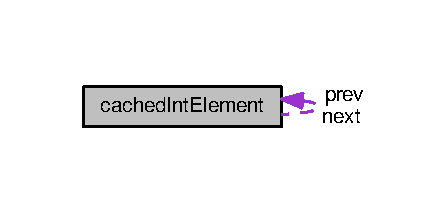
\includegraphics[width=215pt]{structcachedIntElement__coll__graph}
\end{center}
\end{figure}
\subsection*{Public Attributes}
\begin{DoxyCompactItemize}
\item 
uint64\+\_\+t {\bfseries id}\hypertarget{structcachedIntElement_acda821458cfe34dda3bff8b7b0373fb9}{}\label{structcachedIntElement_acda821458cfe34dda3bff8b7b0373fb9}

\item 
uint64\+\_\+t {\bfseries hash}\hypertarget{structcachedIntElement_a20d62592d37c7e8c91449f534431aeb9}{}\label{structcachedIntElement_a20d62592d37c7e8c91449f534431aeb9}

\item 
\hyperlink{structcachedIntElement}{cached\+Int\+Element} $\ast$ {\bfseries next}\hypertarget{structcachedIntElement_ae64f5fae8aa27243af30ef13cb3ebce6}{}\label{structcachedIntElement_ae64f5fae8aa27243af30ef13cb3ebce6}

\item 
\hyperlink{structcachedIntElement}{cached\+Int\+Element} $\ast$ {\bfseries prev}\hypertarget{structcachedIntElement_a90b30c8883b80e42fbf59fbc1bc8727a}{}\label{structcachedIntElement_a90b30c8883b80e42fbf59fbc1bc8727a}

\end{DoxyCompactItemize}


The documentation for this struct was generated from the following file\+:\begin{DoxyCompactItemize}
\item 
hashtable.\+h\end{DoxyCompactItemize}

\hypertarget{structcachedIntList}{}\section{cached\+Int\+List Struct Reference}
\label{structcachedIntList}\index{cached\+Int\+List@{cached\+Int\+List}}


Collaboration diagram for cached\+Int\+List\+:
\nopagebreak
\begin{figure}[H]
\begin{center}
\leavevmode
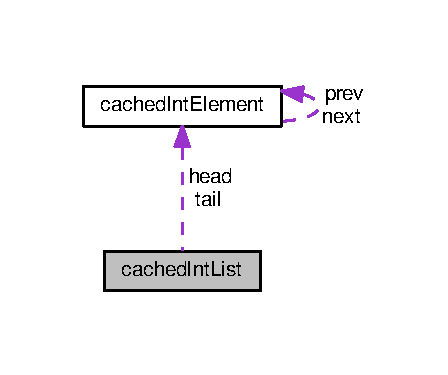
\includegraphics[width=215pt]{structcachedIntList__coll__graph}
\end{center}
\end{figure}
\subsection*{Public Attributes}
\begin{DoxyCompactItemize}
\item 
\hyperlink{structcachedIntElement}{cached\+Int\+Element} $\ast$ {\bfseries head}\hypertarget{structcachedIntList_ac4cce5e5d07c4b23683046e77a0fbe6a}{}\label{structcachedIntList_ac4cce5e5d07c4b23683046e77a0fbe6a}

\item 
\hyperlink{structcachedIntElement}{cached\+Int\+Element} $\ast$ {\bfseries tail}\hypertarget{structcachedIntList_adbe1df126c4425546e3a2b4366784c9d}{}\label{structcachedIntList_adbe1df126c4425546e3a2b4366784c9d}

\end{DoxyCompactItemize}


The documentation for this struct was generated from the following file\+:\begin{DoxyCompactItemize}
\item 
hashtable.\+h\end{DoxyCompactItemize}

\hypertarget{structHashtable}{}\section{Hashtable Struct Reference}
\label{structHashtable}\index{Hashtable@{Hashtable}}


hash table  




{\ttfamily \#include $<$hashtable.\+h$>$}



Collaboration diagram for Hashtable\+:\nopagebreak
\begin{figure}[H]
\begin{center}
\leavevmode
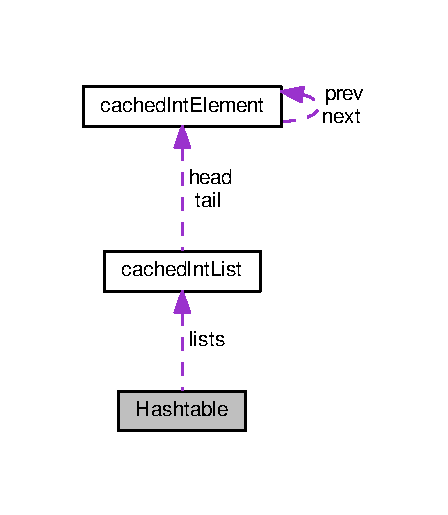
\includegraphics[width=215pt]{structHashtable__coll__graph}
\end{center}
\end{figure}
\subsection*{Public Attributes}
\begin{DoxyCompactItemize}
\item 
int $\ast$ \hyperlink{structHashtable_a99f7c11aa20bbd066528843438a42958}{counter}
\item 
\hyperlink{structcachedIntList}{cached\+Int\+List} $\ast$ \hyperlink{structHashtable_ac4140ebb0209a40547999cce896fe17c}{lists}
\item 
uint64\+\_\+t \hyperlink{structHashtable_aab81586954ce81cc3d52b41cf5ec5a04}{size}
\end{DoxyCompactItemize}


\subsection{Detailed Description}
hash table 

\subsection{Member Data Documentation}
\index{Hashtable@{Hashtable}!counter@{counter}}
\index{counter@{counter}!Hashtable@{Hashtable}}
\subsubsection[{\texorpdfstring{counter}{counter}}]{\setlength{\rightskip}{0pt plus 5cm}int$\ast$ Hashtable\+::counter}\hypertarget{structHashtable_a99f7c11aa20bbd066528843438a42958}{}\label{structHashtable_a99f7c11aa20bbd066528843438a42958}
array of counters of elements in each list \index{Hashtable@{Hashtable}!lists@{lists}}
\index{lists@{lists}!Hashtable@{Hashtable}}
\subsubsection[{\texorpdfstring{lists}{lists}}]{\setlength{\rightskip}{0pt plus 5cm}{\bf cached\+Int\+List}$\ast$ Hashtable\+::lists}\hypertarget{structHashtable_ac4140ebb0209a40547999cce896fe17c}{}\label{structHashtable_ac4140ebb0209a40547999cce896fe17c}
array of lists \index{Hashtable@{Hashtable}!size@{size}}
\index{size@{size}!Hashtable@{Hashtable}}
\subsubsection[{\texorpdfstring{size}{size}}]{\setlength{\rightskip}{0pt plus 5cm}uint64\+\_\+t Hashtable\+::size}\hypertarget{structHashtable_aab81586954ce81cc3d52b41cf5ec5a04}{}\label{structHashtable_aab81586954ce81cc3d52b41cf5ec5a04}
number of lists, size of hash table 

The documentation for this struct was generated from the following file\+:\begin{DoxyCompactItemize}
\item 
\hyperlink{hashtable_8h}{hashtable.\+h}\end{DoxyCompactItemize}

\hypertarget{structMasterCache}{}\section{Master\+Cache Struct Reference}
\label{structMasterCache}\index{Master\+Cache@{Master\+Cache}}


\hyperlink{structMasterCache}{Master\+Cache}.  




{\ttfamily \#include $<$mastercache.\+h$>$}



Collaboration diagram for Master\+Cache\+:\nopagebreak
\begin{figure}[H]
\begin{center}
\leavevmode
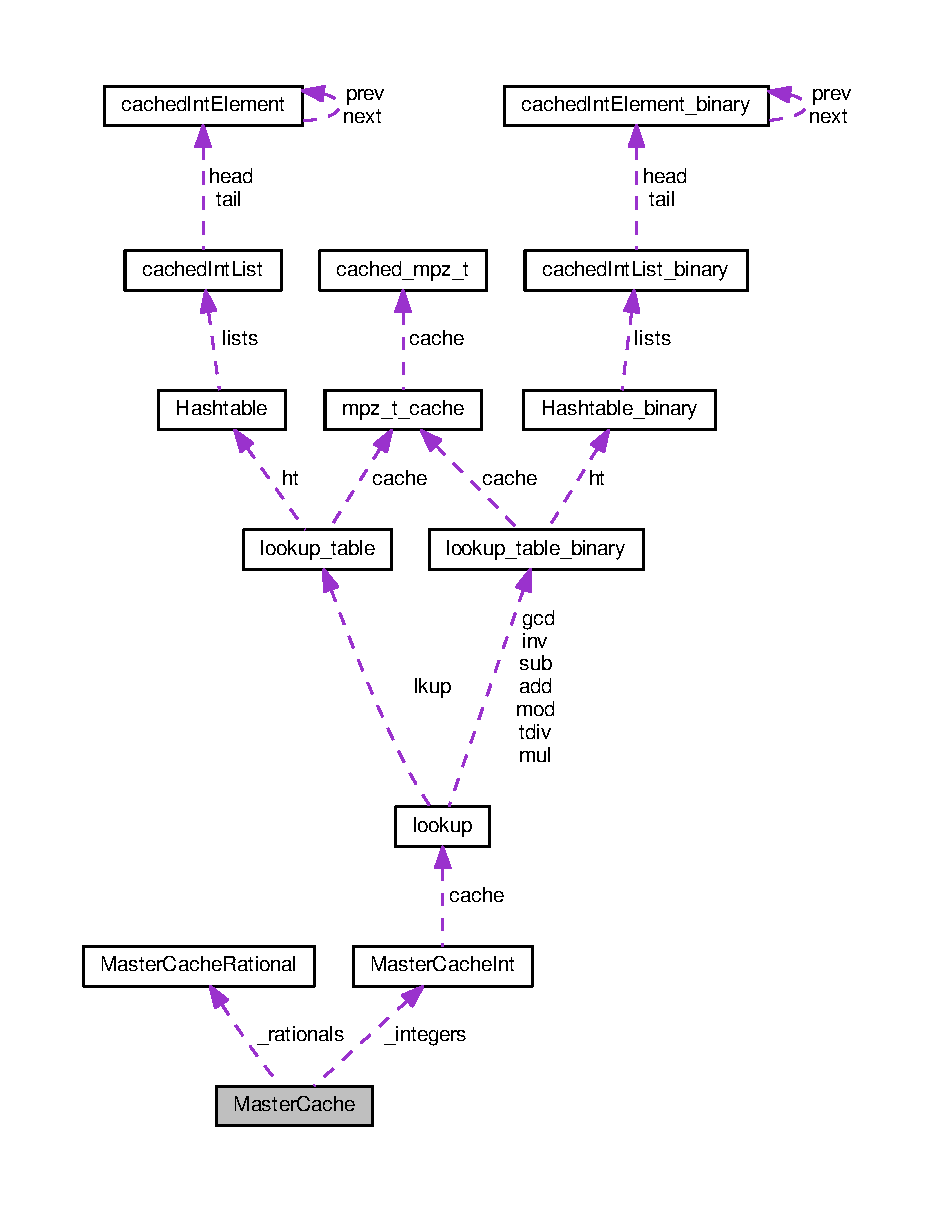
\includegraphics[width=350pt]{structMasterCache__coll__graph}
\end{center}
\end{figure}
\subsection*{Public Attributes}
\begin{DoxyCompactItemize}
\item 
\hyperlink{structMasterCacheInt}{Master\+Cache\+Int} $\ast$ \hyperlink{structMasterCache_a5c3a0aa848b8d98114902f674e111dc3}{\+\_\+integers}
\item 
\hyperlink{structMasterCacheRational}{Master\+Cache\+Rational} $\ast$ \hyperlink{structMasterCache_a2cc414dcdfc90d3841ffa329f0877f67}{\+\_\+rationals}
\end{DoxyCompactItemize}


\subsection{Detailed Description}
\hyperlink{structMasterCache}{Master\+Cache}. 

\subsection{Member Data Documentation}
\index{Master\+Cache@{Master\+Cache}!\+\_\+integers@{\+\_\+integers}}
\index{\+\_\+integers@{\+\_\+integers}!Master\+Cache@{Master\+Cache}}
\subsubsection[{\texorpdfstring{\+\_\+integers}{_integers}}]{\setlength{\rightskip}{0pt plus 5cm}{\bf Master\+Cache\+Int}$\ast$ Master\+Cache\+::\+\_\+integers}\hypertarget{structMasterCache_a5c3a0aa848b8d98114902f674e111dc3}{}\label{structMasterCache_a5c3a0aa848b8d98114902f674e111dc3}
cache for integer caching \index{Master\+Cache@{Master\+Cache}!\+\_\+rationals@{\+\_\+rationals}}
\index{\+\_\+rationals@{\+\_\+rationals}!Master\+Cache@{Master\+Cache}}
\subsubsection[{\texorpdfstring{\+\_\+rationals}{_rationals}}]{\setlength{\rightskip}{0pt plus 5cm}{\bf Master\+Cache\+Rational}$\ast$ Master\+Cache\+::\+\_\+rationals}\hypertarget{structMasterCache_a2cc414dcdfc90d3841ffa329f0877f67}{}\label{structMasterCache_a2cc414dcdfc90d3841ffa329f0877f67}
cache for rational caching 

The documentation for this struct was generated from the following file\+:\begin{DoxyCompactItemize}
\item 
\hyperlink{mastercache_8h}{mastercache.\+h}\end{DoxyCompactItemize}

\hypertarget{structMasterCacheRational}{}\section{Master\+Cache\+Rational Struct Reference}
\label{structMasterCacheRational}\index{Master\+Cache\+Rational@{Master\+Cache\+Rational}}


The documentation for this struct was generated from the following file\+:\begin{DoxyCompactItemize}
\item 
master\+\_\+cache\+\_\+rational.\+c\end{DoxyCompactItemize}

\chapter{File Documentation}
\hypertarget{hashtable_8c}{}\section{hashtable.\+c File Reference}
\label{hashtable_8c}\index{hashtable.\+c@{hashtable.\+c}}


hash table implementation  


{\ttfamily \#include \char`\"{}hashtable.\+h\char`\"{}}\\*
{\ttfamily \#include \char`\"{}hashing.\+h\char`\"{}}\\*
{\ttfamily \#include \char`\"{}mpz\+\_\+caching.\+h\char`\"{}}\\*
{\ttfamily \#include $<$stdint.\+h$>$}\\*
{\ttfamily \#include $<$stdlib.\+h$>$}\\*
{\ttfamily \#include $<$stdio.\+h$>$}\\*
{\ttfamily \#include $<$inttypes.\+h$>$}\\*
Include dependency graph for hashtable.\+c\+:\nopagebreak
\begin{figure}[H]
\begin{center}
\leavevmode
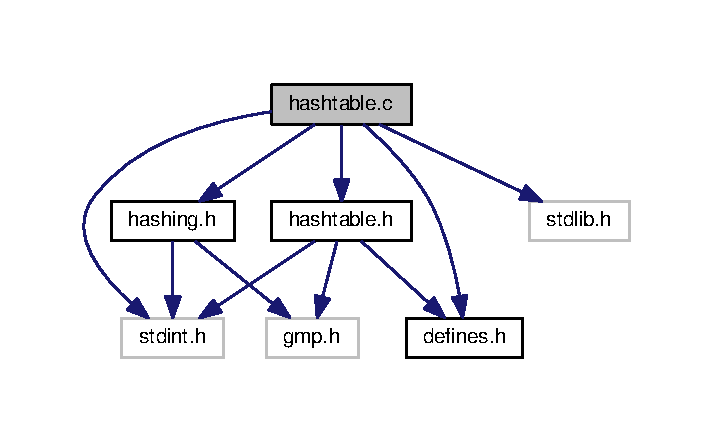
\includegraphics[width=350pt]{hashtable_8c__incl}
\end{center}
\end{figure}
\subsection*{Functions}
\begin{DoxyCompactItemize}
\item 
void \hyperlink{hashtable_8c_a8f4aa8473391505b303072098b101285}{init\+\_\+hashtable} (\hyperlink{structHashtable}{Hashtable} $\ast$ht, uint64\+\_\+t size)
\begin{DoxyCompactList}\small\item\em initialization of the hash table \end{DoxyCompactList}\item 
void \hyperlink{hashtable_8c_a31e50f67c07fb1a475268694bfd5743d}{delete\+\_\+hashtable} (\hyperlink{structHashtable}{Hashtable} $\ast$ht)
\begin{DoxyCompactList}\small\item\em deletion of the hash table and all its underlying data structures \end{DoxyCompactList}\item 
void \hyperlink{hashtable_8c_a3999323c0facade24699b869058ddeb7}{insert\+\_\+element} (\hyperlink{structHashtable}{Hashtable} $\ast$ht, uint64\+\_\+t id, uint64\+\_\+t $\ast$hashes)
\begin{DoxyCompactList}\small\item\em insertion method for an element in the hash table \end{DoxyCompactList}\item 
uint64\+\_\+t \hyperlink{hashtable_8c_aa2cdb80b044d66f091e6cad114e633b9}{exists\+\_\+element} (\hyperlink{structHashtable}{Hashtable} $\ast$ht, uint64\+\_\+t $\ast$hashes, mpz\+\_\+t element, \hyperlink{structmpz__t__cache}{mpz\+\_\+t\+\_\+cache} $\ast$cache)
\begin{DoxyCompactList}\small\item\em check existence of an element \end{DoxyCompactList}\item 
void \hyperlink{hashtable_8c_a7198d8653365a8e7b187bbcb49bab4aa}{get\+\_\+k\+\_\+hashes} (mpz\+\_\+t val, uint64\+\_\+t $\ast$hashes)
\begin{DoxyCompactList}\small\item\em function to calculate the multiple hash values for an mpz\+\_\+t element \end{DoxyCompactList}\item 
void \hyperlink{hashtable_8c_af267b5c3e0669ad9844482299eb9dce0}{get\+\_\+k\+\_\+hashes\+\_\+cpf} (mpz\+\_\+t val1, mpz\+\_\+t val2, uint64\+\_\+t $\ast$hashes)
\begin{DoxyCompactList}\small\item\em function to calculate multiple hashes for a tupel of mpz\+\_\+t\textquotesingle{}s after applying Cantor Pairing function \end{DoxyCompactList}\item 
void \hyperlink{hashtable_8c_a1758c25104d2433ec0fb68861baaa330}{init\+\_\+hashtable\+\_\+binary} (\hyperlink{structHashtable__binary}{Hashtable\+\_\+binary} $\ast$ht, uint64\+\_\+t size)
\begin{DoxyCompactList}\small\item\em initialization of a hashtable for (mpz\+\_\+t x mpz\+\_\+t) -\/$>$ mpz\+\_\+t \end{DoxyCompactList}\item 
void \hyperlink{hashtable_8c_a99e3e52694edc6e5396bc93bcdb2d0eb}{delete\+\_\+hashtable\+\_\+binary} (\hyperlink{structHashtable__binary}{Hashtable\+\_\+binary} $\ast$ht)
\begin{DoxyCompactList}\small\item\em deletion of hash table and all underlying data structures \end{DoxyCompactList}\item 
void \hyperlink{hashtable_8c_a8d6049bccb0ee7c582dd8190c9e0530d}{insert\+\_\+element\+\_\+binary} (\hyperlink{structHashtable__binary}{Hashtable\+\_\+binary} $\ast$ht, uint64\+\_\+t id\+\_\+op1, uint64\+\_\+t id\+\_\+op2, uint64\+\_\+t id\+\_\+res, uint64\+\_\+t $\ast$extra\+\_\+info, uint64\+\_\+t $\ast$hashes)
\begin{DoxyCompactList}\small\item\em insert a mapping (mpz\+\_\+t x mpz\+\_\+t) -\/$>$ mpz\+\_\+t in hashtable \end{DoxyCompactList}\item 
uint64\+\_\+t \hyperlink{hashtable_8c_a640832720182207089e4e7156ffcac6d}{exists\+\_\+element\+\_\+binary} (\hyperlink{structHashtable__binary}{Hashtable\+\_\+binary} $\ast$ht, uint64\+\_\+t $\ast$hashes, mpz\+\_\+t op1, mpz\+\_\+t op2, \hyperlink{structmpz__t__cache}{mpz\+\_\+t\+\_\+cache} $\ast$cache, uint64\+\_\+t $\ast$extra\+\_\+info)
\begin{DoxyCompactList}\small\item\em function to check if a mapping (mpz\+\_\+t x mpz\+\_\+t) -\/$>$ mpz\+\_\+t exists in the hash table \end{DoxyCompactList}\end{DoxyCompactItemize}


\subsection{Detailed Description}
hash table implementation 

\begin{DoxyAuthor}{Author}
Sandra Hicks 
\end{DoxyAuthor}


\subsection{Function Documentation}
\index{hashtable.\+c@{hashtable.\+c}!delete\+\_\+hashtable@{delete\+\_\+hashtable}}
\index{delete\+\_\+hashtable@{delete\+\_\+hashtable}!hashtable.\+c@{hashtable.\+c}}
\subsubsection[{\texorpdfstring{delete\+\_\+hashtable(\+Hashtable $\ast$ht)}{delete_hashtable(Hashtable *ht)}}]{\setlength{\rightskip}{0pt plus 5cm}void delete\+\_\+hashtable (
\begin{DoxyParamCaption}
\item[{{\bf Hashtable} $\ast$}]{ht}
\end{DoxyParamCaption}
)}\hypertarget{hashtable_8c_a31e50f67c07fb1a475268694bfd5743d}{}\label{hashtable_8c_a31e50f67c07fb1a475268694bfd5743d}


deletion of the hash table and all its underlying data structures 


\begin{DoxyParams}{Parameters}
{\em ht} & pointer to hash table \\
\hline
\end{DoxyParams}
\index{hashtable.\+c@{hashtable.\+c}!delete\+\_\+hashtable\+\_\+binary@{delete\+\_\+hashtable\+\_\+binary}}
\index{delete\+\_\+hashtable\+\_\+binary@{delete\+\_\+hashtable\+\_\+binary}!hashtable.\+c@{hashtable.\+c}}
\subsubsection[{\texorpdfstring{delete\+\_\+hashtable\+\_\+binary(\+Hashtable\+\_\+binary $\ast$ht)}{delete_hashtable_binary(Hashtable_binary *ht)}}]{\setlength{\rightskip}{0pt plus 5cm}void delete\+\_\+hashtable\+\_\+binary (
\begin{DoxyParamCaption}
\item[{{\bf Hashtable\+\_\+binary} $\ast$}]{ht}
\end{DoxyParamCaption}
)}\hypertarget{hashtable_8c_a99e3e52694edc6e5396bc93bcdb2d0eb}{}\label{hashtable_8c_a99e3e52694edc6e5396bc93bcdb2d0eb}


deletion of hash table and all underlying data structures 


\begin{DoxyParams}{Parameters}
{\em ht} & pointer to hash table \\
\hline
\end{DoxyParams}
\index{hashtable.\+c@{hashtable.\+c}!exists\+\_\+element@{exists\+\_\+element}}
\index{exists\+\_\+element@{exists\+\_\+element}!hashtable.\+c@{hashtable.\+c}}
\subsubsection[{\texorpdfstring{exists\+\_\+element(\+Hashtable $\ast$ht, uint64\+\_\+t $\ast$hashes, mpz\+\_\+t element, mpz\+\_\+t\+\_\+cache $\ast$cache)}{exists_element(Hashtable *ht, uint64_t *hashes, mpz_t element, mpz_t_cache *cache)}}]{\setlength{\rightskip}{0pt plus 5cm}uint64\+\_\+t exists\+\_\+element (
\begin{DoxyParamCaption}
\item[{{\bf Hashtable} $\ast$}]{ht, }
\item[{uint64\+\_\+t $\ast$}]{hashes, }
\item[{mpz\+\_\+t}]{element, }
\item[{{\bf mpz\+\_\+t\+\_\+cache} $\ast$}]{cache}
\end{DoxyParamCaption}
)}\hypertarget{hashtable_8c_aa2cdb80b044d66f091e6cad114e633b9}{}\label{hashtable_8c_aa2cdb80b044d66f091e6cad114e633b9}


check existence of an element 


\begin{DoxyParams}{Parameters}
{\em ht} & pointer to hash table \\
\hline
{\em hashes} & array of hash values for the element \\
\hline
{\em element} & mpz\+\_\+t to search for \\
\hline
{\em cache} & pointer to singleton cache \\
\hline
\end{DoxyParams}
\begin{DoxyReturn}{Returns}
id if existent, if not return 0 
\end{DoxyReturn}
\index{hashtable.\+c@{hashtable.\+c}!exists\+\_\+element\+\_\+binary@{exists\+\_\+element\+\_\+binary}}
\index{exists\+\_\+element\+\_\+binary@{exists\+\_\+element\+\_\+binary}!hashtable.\+c@{hashtable.\+c}}
\subsubsection[{\texorpdfstring{exists\+\_\+element\+\_\+binary(\+Hashtable\+\_\+binary $\ast$ht, uint64\+\_\+t $\ast$hashes, mpz\+\_\+t op1, mpz\+\_\+t op2, mpz\+\_\+t\+\_\+cache $\ast$cache, uint64\+\_\+t $\ast$extra\+\_\+info)}{exists_element_binary(Hashtable_binary *ht, uint64_t *hashes, mpz_t op1, mpz_t op2, mpz_t_cache *cache, uint64_t *extra_info)}}]{\setlength{\rightskip}{0pt plus 5cm}uint64\+\_\+t exists\+\_\+element\+\_\+binary (
\begin{DoxyParamCaption}
\item[{{\bf Hashtable\+\_\+binary} $\ast$}]{ht, }
\item[{uint64\+\_\+t $\ast$}]{hashes, }
\item[{mpz\+\_\+t}]{op1, }
\item[{mpz\+\_\+t}]{op2, }
\item[{{\bf mpz\+\_\+t\+\_\+cache} $\ast$}]{cache, }
\item[{uint64\+\_\+t $\ast$}]{extra\+\_\+info}
\end{DoxyParamCaption}
)}\hypertarget{hashtable_8c_a640832720182207089e4e7156ffcac6d}{}\label{hashtable_8c_a640832720182207089e4e7156ffcac6d}


function to check if a mapping (mpz\+\_\+t x mpz\+\_\+t) -\/$>$ mpz\+\_\+t exists in the hash table 


\begin{DoxyParams}{Parameters}
{\em ht} & pointer to hash table \\
\hline
{\em hashes} & array of hashes \\
\hline
{\em op1} & first operator \\
\hline
{\em op2} & second operator \\
\hline
{\em cache} & pointer to singleton mpz\+\_\+t cache \\
\hline
{\em extra\+\_\+info} & id of extra info of found element, stays null if none exists \\
\hline
\end{DoxyParams}
\begin{DoxyReturn}{Returns}
id if found, 0 if not existent 
\end{DoxyReturn}
\index{hashtable.\+c@{hashtable.\+c}!get\+\_\+k\+\_\+hashes@{get\+\_\+k\+\_\+hashes}}
\index{get\+\_\+k\+\_\+hashes@{get\+\_\+k\+\_\+hashes}!hashtable.\+c@{hashtable.\+c}}
\subsubsection[{\texorpdfstring{get\+\_\+k\+\_\+hashes(mpz\+\_\+t val, uint64\+\_\+t $\ast$hashes)}{get_k_hashes(mpz_t val, uint64_t *hashes)}}]{\setlength{\rightskip}{0pt plus 5cm}void get\+\_\+k\+\_\+hashes (
\begin{DoxyParamCaption}
\item[{mpz\+\_\+t}]{val, }
\item[{uint64\+\_\+t $\ast$}]{hashes}
\end{DoxyParamCaption}
)}\hypertarget{hashtable_8c_a7198d8653365a8e7b187bbcb49bab4aa}{}\label{hashtable_8c_a7198d8653365a8e7b187bbcb49bab4aa}


function to calculate the multiple hash values for an mpz\+\_\+t element 


\begin{DoxyParams}{Parameters}
{\em val} & mpz\+\_\+t value to hash \\
\hline
{\em hashes} & pointer to array of hashes to fill \\
\hline
\end{DoxyParams}
\index{hashtable.\+c@{hashtable.\+c}!get\+\_\+k\+\_\+hashes\+\_\+cpf@{get\+\_\+k\+\_\+hashes\+\_\+cpf}}
\index{get\+\_\+k\+\_\+hashes\+\_\+cpf@{get\+\_\+k\+\_\+hashes\+\_\+cpf}!hashtable.\+c@{hashtable.\+c}}
\subsubsection[{\texorpdfstring{get\+\_\+k\+\_\+hashes\+\_\+cpf(mpz\+\_\+t val1, mpz\+\_\+t val2, uint64\+\_\+t $\ast$hashes)}{get_k_hashes_cpf(mpz_t val1, mpz_t val2, uint64_t *hashes)}}]{\setlength{\rightskip}{0pt plus 5cm}void get\+\_\+k\+\_\+hashes\+\_\+cpf (
\begin{DoxyParamCaption}
\item[{mpz\+\_\+t}]{val1, }
\item[{mpz\+\_\+t}]{val2, }
\item[{uint64\+\_\+t $\ast$}]{hashes}
\end{DoxyParamCaption}
)}\hypertarget{hashtable_8c_af267b5c3e0669ad9844482299eb9dce0}{}\label{hashtable_8c_af267b5c3e0669ad9844482299eb9dce0}


function to calculate multiple hashes for a tupel of mpz\+\_\+t\textquotesingle{}s after applying Cantor Pairing function 


\begin{DoxyParams}{Parameters}
{\em val1} & first mpz\+\_\+t \\
\hline
{\em val2} & second mpz\+\_\+t \\
\hline
{\em hashes} & array of hashes to fill \\
\hline
\end{DoxyParams}
\index{hashtable.\+c@{hashtable.\+c}!init\+\_\+hashtable@{init\+\_\+hashtable}}
\index{init\+\_\+hashtable@{init\+\_\+hashtable}!hashtable.\+c@{hashtable.\+c}}
\subsubsection[{\texorpdfstring{init\+\_\+hashtable(\+Hashtable $\ast$ht, uint64\+\_\+t size)}{init_hashtable(Hashtable *ht, uint64_t size)}}]{\setlength{\rightskip}{0pt plus 5cm}void init\+\_\+hashtable (
\begin{DoxyParamCaption}
\item[{{\bf Hashtable} $\ast$}]{ht, }
\item[{uint64\+\_\+t}]{size}
\end{DoxyParamCaption}
)}\hypertarget{hashtable_8c_a8f4aa8473391505b303072098b101285}{}\label{hashtable_8c_a8f4aa8473391505b303072098b101285}


initialization of the hash table 


\begin{DoxyParams}{Parameters}
{\em ht} & pointer to hash table \\
\hline
{\em size} & of the hash table \\
\hline
\end{DoxyParams}
\index{hashtable.\+c@{hashtable.\+c}!init\+\_\+hashtable\+\_\+binary@{init\+\_\+hashtable\+\_\+binary}}
\index{init\+\_\+hashtable\+\_\+binary@{init\+\_\+hashtable\+\_\+binary}!hashtable.\+c@{hashtable.\+c}}
\subsubsection[{\texorpdfstring{init\+\_\+hashtable\+\_\+binary(\+Hashtable\+\_\+binary $\ast$ht, uint64\+\_\+t size)}{init_hashtable_binary(Hashtable_binary *ht, uint64_t size)}}]{\setlength{\rightskip}{0pt plus 5cm}void init\+\_\+hashtable\+\_\+binary (
\begin{DoxyParamCaption}
\item[{{\bf Hashtable\+\_\+binary} $\ast$}]{ht, }
\item[{uint64\+\_\+t}]{size}
\end{DoxyParamCaption}
)}\hypertarget{hashtable_8c_a1758c25104d2433ec0fb68861baaa330}{}\label{hashtable_8c_a1758c25104d2433ec0fb68861baaa330}


initialization of a hashtable for (mpz\+\_\+t x mpz\+\_\+t) -\/$>$ mpz\+\_\+t 


\begin{DoxyParams}{Parameters}
{\em ht} & pointer to hash table \\
\hline
{\em size} & size of hash table \\
\hline
\end{DoxyParams}
\index{hashtable.\+c@{hashtable.\+c}!insert\+\_\+element@{insert\+\_\+element}}
\index{insert\+\_\+element@{insert\+\_\+element}!hashtable.\+c@{hashtable.\+c}}
\subsubsection[{\texorpdfstring{insert\+\_\+element(\+Hashtable $\ast$ht, uint64\+\_\+t id, uint64\+\_\+t $\ast$hashes)}{insert_element(Hashtable *ht, uint64_t id, uint64_t *hashes)}}]{\setlength{\rightskip}{0pt plus 5cm}void insert\+\_\+element (
\begin{DoxyParamCaption}
\item[{{\bf Hashtable} $\ast$}]{ht, }
\item[{uint64\+\_\+t}]{id, }
\item[{uint64\+\_\+t $\ast$}]{hashes}
\end{DoxyParamCaption}
)}\hypertarget{hashtable_8c_a3999323c0facade24699b869058ddeb7}{}\label{hashtable_8c_a3999323c0facade24699b869058ddeb7}


insertion method for an element in the hash table 


\begin{DoxyParams}{Parameters}
{\em ht} & pointer to hash table \\
\hline
{\em id} & id of the mpz\+\_\+t in the singleton cache \\
\hline
{\em hashes} & array of hash values of the mpz\+\_\+t \\
\hline
\end{DoxyParams}
\index{hashtable.\+c@{hashtable.\+c}!insert\+\_\+element\+\_\+binary@{insert\+\_\+element\+\_\+binary}}
\index{insert\+\_\+element\+\_\+binary@{insert\+\_\+element\+\_\+binary}!hashtable.\+c@{hashtable.\+c}}
\subsubsection[{\texorpdfstring{insert\+\_\+element\+\_\+binary(\+Hashtable\+\_\+binary $\ast$ht, uint64\+\_\+t id\+\_\+op1, uint64\+\_\+t id\+\_\+op2, uint64\+\_\+t id\+\_\+res, uint64\+\_\+t $\ast$extra\+\_\+info, uint64\+\_\+t $\ast$hashes)}{insert_element_binary(Hashtable_binary *ht, uint64_t id_op1, uint64_t id_op2, uint64_t id_res, uint64_t *extra_info, uint64_t *hashes)}}]{\setlength{\rightskip}{0pt plus 5cm}void insert\+\_\+element\+\_\+binary (
\begin{DoxyParamCaption}
\item[{{\bf Hashtable\+\_\+binary} $\ast$}]{ht, }
\item[{uint64\+\_\+t}]{id\+\_\+op1, }
\item[{uint64\+\_\+t}]{id\+\_\+op2, }
\item[{uint64\+\_\+t}]{id\+\_\+res, }
\item[{uint64\+\_\+t $\ast$}]{extra\+\_\+info, }
\item[{uint64\+\_\+t $\ast$}]{hashes}
\end{DoxyParamCaption}
)}\hypertarget{hashtable_8c_a8d6049bccb0ee7c582dd8190c9e0530d}{}\label{hashtable_8c_a8d6049bccb0ee7c582dd8190c9e0530d}


insert a mapping (mpz\+\_\+t x mpz\+\_\+t) -\/$>$ mpz\+\_\+t in hashtable 


\begin{DoxyParams}{Parameters}
{\em ht} & pointer to hash table \\
\hline
{\em id\+\_\+op1} & id to first operand in singleton cache \\
\hline
{\em id\+\_\+op2} & id to second operand in singleton cache \\
\hline
{\em id\+\_\+res} & id to result in singleton cache \\
\hline
{\em extra\+\_\+info} & id to extra info in singleton cache (e.\+g. division rest) \\
\hline
{\em hashes} & array of hashes \\
\hline
\end{DoxyParams}

\hypertarget{master__cache__integer_8c}{}\section{master\+\_\+cache\+\_\+integer.\+c File Reference}
\label{master__cache__integer_8c}\index{master\+\_\+cache\+\_\+integer.\+c@{master\+\_\+cache\+\_\+integer.\+c}}


Master Cache functions for caching Integer operations in gmp.  


{\ttfamily \#include $<$stdint.\+h$>$}\\*
{\ttfamily \#include $<$gmp.\+h$>$}\\*
{\ttfamily \#include $<$limits.\+h$>$}\\*
{\ttfamily \#include $<$stdlib.\+h$>$}\\*
{\ttfamily \#include $<$float.\+h$>$}\\*
{\ttfamily \#include \char`\"{}mastercache.\+h\char`\"{}}\\*
{\ttfamily \#include \char`\"{}master\+\_\+cache\+\_\+integer.\+h\char`\"{}}\\*
{\ttfamily \#include \char`\"{}caching\+\_\+operations.\+h\char`\"{}}\\*
{\ttfamily \#include \char`\"{}overflow\+\_\+detection.\+h\char`\"{}}\\*
{\ttfamily \#include $<$stdio.\+h$>$}\\*
{\ttfamily \#include $<$inttypes.\+h$>$}\\*
Include dependency graph for master\+\_\+cache\+\_\+integer.\+c\+:\nopagebreak
\begin{figure}[H]
\begin{center}
\leavevmode
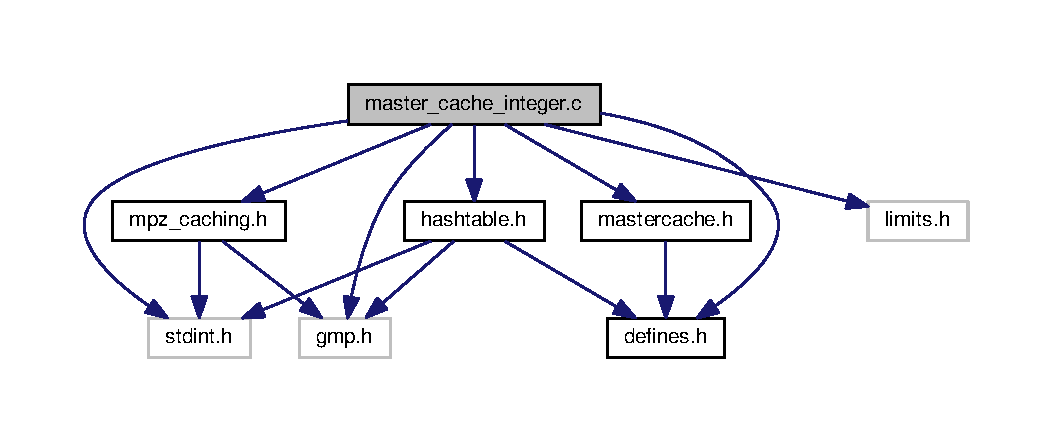
\includegraphics[width=350pt]{master__cache__integer_8c__incl}
\end{center}
\end{figure}
\subsection*{Functions}
\begin{DoxyCompactItemize}
\item 
\hyperlink{mastercache_8h_a113c03970467afb459ed5ae157d0a870}{cached\+Int} \hyperlink{master__cache__integer_8c_acf48c6c064be125bfc2e3daf62f10177}{direct\+\_\+add} (\hyperlink{mastercache_8h_a113c03970467afb459ed5ae157d0a870}{cached\+Int} val1, \hyperlink{mastercache_8h_a113c03970467afb459ed5ae157d0a870}{cached\+Int} val2)
\item 
\hyperlink{mastercache_8h_a113c03970467afb459ed5ae157d0a870}{cached\+Int} \hyperlink{master__cache__integer_8c_aa558a557fa5371fc35597dc52fd824e5}{direct\+\_\+mul} (\hyperlink{mastercache_8h_a113c03970467afb459ed5ae157d0a870}{cached\+Int} val1, \hyperlink{mastercache_8h_a113c03970467afb459ed5ae157d0a870}{cached\+Int} val2)
\item 
\hyperlink{mastercache_8h_a113c03970467afb459ed5ae157d0a870}{cached\+Int} \hyperlink{master__cache__integer_8c_a7cbe579aa33d35c4042fac942fed2070}{direct\+\_\+div} (\hyperlink{mastercache_8h_a113c03970467afb459ed5ae157d0a870}{cached\+Int} val1, \hyperlink{mastercache_8h_a113c03970467afb459ed5ae157d0a870}{cached\+Int} val2)
\item 
\hyperlink{mastercache_8h_a113c03970467afb459ed5ae157d0a870}{cached\+Int} \hyperlink{master__cache__integer_8c_abe0e4d423323534bba705a0e6fed30dc}{direct\+\_\+mod} (\hyperlink{mastercache_8h_a113c03970467afb459ed5ae157d0a870}{cached\+Int} val1, \hyperlink{mastercache_8h_a113c03970467afb459ed5ae157d0a870}{cached\+Int} val2)
\item 
\hyperlink{mastercache_8h_a113c03970467afb459ed5ae157d0a870}{cached\+Int} \hyperlink{master__cache__integer_8c_a663303ff03efc5249b8aa408ff5cce29}{direct\+\_\+gcd} (\hyperlink{mastercache_8h_a113c03970467afb459ed5ae157d0a870}{cached\+Int} val1, \hyperlink{mastercache_8h_a113c03970467afb459ed5ae157d0a870}{cached\+Int} val2)
\item 
\hyperlink{mastercache_8h_a113c03970467afb459ed5ae157d0a870}{cached\+Int} \hyperlink{master__cache__integer_8c_aae7d64a848078cd497869680dbca4780}{direct\+\_\+invert} (\hyperlink{mastercache_8h_a113c03970467afb459ed5ae157d0a870}{cached\+Int} val1, \hyperlink{mastercache_8h_a113c03970467afb459ed5ae157d0a870}{cached\+Int} val2)
\item 
void \hyperlink{master__cache__integer_8c_a66c8c57579e8806ff904aeb71d54ec44}{ext\+\_\+euclid} (\hyperlink{mastercache_8h_a113c03970467afb459ed5ae157d0a870}{cached\+Int} val1, \hyperlink{mastercache_8h_a113c03970467afb459ed5ae157d0a870}{cached\+Int} val2, \hyperlink{mastercache_8h_a113c03970467afb459ed5ae157d0a870}{cached\+Int} $\ast$d, \hyperlink{mastercache_8h_a113c03970467afb459ed5ae157d0a870}{cached\+Int} $\ast$s, \hyperlink{mastercache_8h_a113c03970467afb459ed5ae157d0a870}{cached\+Int} $\ast$t)
\item 
void \hyperlink{master__cache__integer_8c_a6095b13ce14cae93851e746599d8038e}{cached\+\_\+int\+\_\+init\+\_\+cache} (\hyperlink{structMasterCache}{Master\+Cache} $\ast$mstr, uint64\+\_\+t cachesize)
\begin{DoxyCompactList}\small\item\em function for master cache to initialize \end{DoxyCompactList}\item 
void \hyperlink{master__cache__integer_8c_a1f693b4093b62e1c70a866b4947cea00}{cached\+\_\+int\+\_\+clear\+\_\+cache} (\hyperlink{structMasterCache}{Master\+Cache} $\ast$mstr)
\begin{DoxyCompactList}\small\item\em function for master cache to clear all background data before free \end{DoxyCompactList}\item 
uint64\+\_\+t \hyperlink{master__cache__integer_8c_a8ad24c72fe1e1e7bcb71342763573276}{mpz\+\_\+cached\+\_\+int} (mpz\+\_\+t number)
\item 
void \hyperlink{master__cache__integer_8c_ac755a7c217e68e03bac95bda3c12e2a7}{cached\+\_\+int\+\_\+mpz} (\hyperlink{mastercache_8h_a113c03970467afb459ed5ae157d0a870}{cached\+Int} id, mpz\+\_\+t number)
\item 
\hyperlink{mastercache_8h_a113c03970467afb459ed5ae157d0a870}{cached\+Int} \hyperlink{master__cache__integer_8c_a2e8ed43761ae3945335b89102db422fd}{cached\+\_\+int\+\_\+set} (\hyperlink{structMasterCache}{Master\+Cache} $\ast$mstr, mpz\+\_\+t number)
\begin{DoxyCompactList}\small\item\em function for master cache to set a mpz\+\_\+t and get back an id \end{DoxyCompactList}\item 
void \hyperlink{master__cache__integer_8c_a70e68c14bd00b07597b31dba34aba997}{cached\+\_\+int\+\_\+get} (\hyperlink{structMasterCache}{Master\+Cache} $\ast$mstr, \hyperlink{mastercache_8h_a113c03970467afb459ed5ae157d0a870}{cached\+Int} id, mpz\+\_\+t number)
\begin{DoxyCompactList}\small\item\em function for master cache to get a previously cached mpz\+\_\+t from an id \end{DoxyCompactList}\item 
double \hyperlink{master__cache__integer_8c_af0c42f55a0674b42df4ce45322c33198}{cached\+\_\+int\+\_\+get\+\_\+d} (\hyperlink{structMasterCache}{Master\+Cache} $\ast$mstr, \hyperlink{mastercache_8h_a113c03970467afb459ed5ae157d0a870}{cached\+Int} id)
\begin{DoxyCompactList}\small\item\em function for master cache to get a previously cached mpz\+\_\+t as double from an id \end{DoxyCompactList}\item 
\hyperlink{mastercache_8h_a113c03970467afb459ed5ae157d0a870}{cached\+Int} \hyperlink{master__cache__integer_8c_a2c77389b27a3a9c47f580cc52b6bbe62}{cached\+\_\+int\+\_\+add} (\hyperlink{structMasterCache}{Master\+Cache} $\ast$mstr, \hyperlink{mastercache_8h_a113c03970467afb459ed5ae157d0a870}{cached\+Int} val1, \hyperlink{mastercache_8h_a113c03970467afb459ed5ae157d0a870}{cached\+Int} val2)
\begin{DoxyCompactList}\small\item\em function for master cache to add two cached values and cache the result if large. \end{DoxyCompactList}\item 
\hyperlink{mastercache_8h_a113c03970467afb459ed5ae157d0a870}{cached\+Int} \hyperlink{master__cache__integer_8c_af3fa99a34d3f8f474ca5cb1caf45b0dc}{cached\+\_\+int\+\_\+sub} (\hyperlink{structMasterCache}{Master\+Cache} $\ast$mstr, \hyperlink{mastercache_8h_a113c03970467afb459ed5ae157d0a870}{cached\+Int} val1, \hyperlink{mastercache_8h_a113c03970467afb459ed5ae157d0a870}{cached\+Int} val2)
\begin{DoxyCompactList}\small\item\em function for master cache to subtract two cached values and cache the result if large. \end{DoxyCompactList}\item 
\hyperlink{mastercache_8h_a113c03970467afb459ed5ae157d0a870}{cached\+Int} \hyperlink{master__cache__integer_8c_a418f697aefb1a082369940b69ef21758}{cached\+\_\+int\+\_\+mul} (\hyperlink{structMasterCache}{Master\+Cache} $\ast$mstr, \hyperlink{mastercache_8h_a113c03970467afb459ed5ae157d0a870}{cached\+Int} val1, \hyperlink{mastercache_8h_a113c03970467afb459ed5ae157d0a870}{cached\+Int} val2)
\begin{DoxyCompactList}\small\item\em function for master cache to multiply two cached values and cache the result if large. \end{DoxyCompactList}\item 
\hyperlink{mastercache_8h_a113c03970467afb459ed5ae157d0a870}{cached\+Int} \hyperlink{master__cache__integer_8c_a65de9b96c7568d2a4bc8a6a05749be04}{cached\+\_\+int\+\_\+tdiv} (\hyperlink{structMasterCache}{Master\+Cache} $\ast$mstr, \hyperlink{mastercache_8h_a113c03970467afb459ed5ae157d0a870}{cached\+Int} divident, \hyperlink{mastercache_8h_a113c03970467afb459ed5ae157d0a870}{cached\+Int} divisor, \hyperlink{mastercache_8h_a113c03970467afb459ed5ae157d0a870}{cached\+Int} $\ast$rest)
\begin{DoxyCompactList}\small\item\em function for master cache to divide two cached values and cache the result if large. \end{DoxyCompactList}\item 
\hyperlink{mastercache_8h_a113c03970467afb459ed5ae157d0a870}{cached\+Int} \hyperlink{master__cache__integer_8c_ac95bf4ec8ac8cdfc09f81dc6ab3f7954}{cached\+\_\+int\+\_\+mod} (\hyperlink{structMasterCache}{Master\+Cache} $\ast$mstr, \hyperlink{mastercache_8h_a113c03970467afb459ed5ae157d0a870}{cached\+Int} number, \hyperlink{mastercache_8h_a113c03970467afb459ed5ae157d0a870}{cached\+Int} n)
\begin{DoxyCompactList}\small\item\em function for master cache to calculate the modulo of two cached values and cache the result if large. \end{DoxyCompactList}\item 
\hyperlink{mastercache_8h_a113c03970467afb459ed5ae157d0a870}{cached\+Int} \hyperlink{master__cache__integer_8c_aee6e62d1fc9500706bd768db8e2a5af3}{cached\+\_\+int\+\_\+gcd} (\hyperlink{structMasterCache}{Master\+Cache} $\ast$mstr, \hyperlink{mastercache_8h_a113c03970467afb459ed5ae157d0a870}{cached\+Int} val1, \hyperlink{mastercache_8h_a113c03970467afb459ed5ae157d0a870}{cached\+Int} val2)
\begin{DoxyCompactList}\small\item\em function for master cache to calculate the greatest common divisor of two cached values and cache the result if large. \end{DoxyCompactList}\item 
int \hyperlink{master__cache__integer_8c_aaabedd43537e5425aebea90933ccaa75}{cached\+\_\+int\+\_\+invert} (\hyperlink{structMasterCache}{Master\+Cache} $\ast$mstr, \hyperlink{mastercache_8h_a113c03970467afb459ed5ae157d0a870}{cached\+Int} val1, \hyperlink{mastercache_8h_a113c03970467afb459ed5ae157d0a870}{cached\+Int} val2, \hyperlink{mastercache_8h_a113c03970467afb459ed5ae157d0a870}{cached\+Int} $\ast$result)
\begin{DoxyCompactList}\small\item\em function for master cache to calculate the inverse of a cached value mod n and cache the result if large. \end{DoxyCompactList}\end{DoxyCompactItemize}


\subsection{Detailed Description}
Master Cache functions for caching Integer operations in gmp. 

\begin{DoxyAuthor}{Author}
Sandra Hicks 
\end{DoxyAuthor}


\subsection{Function Documentation}
\index{master\+\_\+cache\+\_\+integer.\+c@{master\+\_\+cache\+\_\+integer.\+c}!cached\+\_\+int\+\_\+add@{cached\+\_\+int\+\_\+add}}
\index{cached\+\_\+int\+\_\+add@{cached\+\_\+int\+\_\+add}!master\+\_\+cache\+\_\+integer.\+c@{master\+\_\+cache\+\_\+integer.\+c}}
\subsubsection[{\texorpdfstring{cached\+\_\+int\+\_\+add(\+Master\+Cache $\ast$mstr, cached\+Int val1, cached\+Int val2)}{cached_int_add(MasterCache *mstr, cachedInt val1, cachedInt val2)}}]{\setlength{\rightskip}{0pt plus 5cm}{\bf cached\+Int} cached\+\_\+int\+\_\+add (
\begin{DoxyParamCaption}
\item[{{\bf Master\+Cache} $\ast$}]{mstr, }
\item[{{\bf cached\+Int}}]{val1, }
\item[{{\bf cached\+Int}}]{val2}
\end{DoxyParamCaption}
)}\hypertarget{master__cache__integer_8c_a2c77389b27a3a9c47f580cc52b6bbe62}{}\label{master__cache__integer_8c_a2c77389b27a3a9c47f580cc52b6bbe62}


function for master cache to add two cached values and cache the result if large. 


\begin{DoxyParams}{Parameters}
{\em mstr} & \hyperlink{structMasterCache}{Master\+Cache} pointer \\
\hline
{\em val1} & id of the first operand \\
\hline
{\em val2} & id of the second operand \\
\hline
\end{DoxyParams}
\begin{DoxyReturn}{Returns}
cached\+Int returns caching id or result for addtion 
\end{DoxyReturn}
\index{master\+\_\+cache\+\_\+integer.\+c@{master\+\_\+cache\+\_\+integer.\+c}!cached\+\_\+int\+\_\+clear\+\_\+cache@{cached\+\_\+int\+\_\+clear\+\_\+cache}}
\index{cached\+\_\+int\+\_\+clear\+\_\+cache@{cached\+\_\+int\+\_\+clear\+\_\+cache}!master\+\_\+cache\+\_\+integer.\+c@{master\+\_\+cache\+\_\+integer.\+c}}
\subsubsection[{\texorpdfstring{cached\+\_\+int\+\_\+clear\+\_\+cache(\+Master\+Cache $\ast$mstr)}{cached_int_clear_cache(MasterCache *mstr)}}]{\setlength{\rightskip}{0pt plus 5cm}void cached\+\_\+int\+\_\+clear\+\_\+cache (
\begin{DoxyParamCaption}
\item[{{\bf Master\+Cache} $\ast$}]{mstr}
\end{DoxyParamCaption}
)}\hypertarget{master__cache__integer_8c_a1f693b4093b62e1c70a866b4947cea00}{}\label{master__cache__integer_8c_a1f693b4093b62e1c70a866b4947cea00}


function for master cache to clear all background data before free 


\begin{DoxyParams}{Parameters}
{\em mstr} & \hyperlink{structMasterCache}{Master\+Cache} pointer \\
\hline
\end{DoxyParams}
\index{master\+\_\+cache\+\_\+integer.\+c@{master\+\_\+cache\+\_\+integer.\+c}!cached\+\_\+int\+\_\+gcd@{cached\+\_\+int\+\_\+gcd}}
\index{cached\+\_\+int\+\_\+gcd@{cached\+\_\+int\+\_\+gcd}!master\+\_\+cache\+\_\+integer.\+c@{master\+\_\+cache\+\_\+integer.\+c}}
\subsubsection[{\texorpdfstring{cached\+\_\+int\+\_\+gcd(\+Master\+Cache $\ast$mstr, cached\+Int val1, cached\+Int val2)}{cached_int_gcd(MasterCache *mstr, cachedInt val1, cachedInt val2)}}]{\setlength{\rightskip}{0pt plus 5cm}{\bf cached\+Int} cached\+\_\+int\+\_\+gcd (
\begin{DoxyParamCaption}
\item[{{\bf Master\+Cache} $\ast$}]{mstr, }
\item[{{\bf cached\+Int}}]{val1, }
\item[{{\bf cached\+Int}}]{val2}
\end{DoxyParamCaption}
)}\hypertarget{master__cache__integer_8c_aee6e62d1fc9500706bd768db8e2a5af3}{}\label{master__cache__integer_8c_aee6e62d1fc9500706bd768db8e2a5af3}


function for master cache to calculate the greatest common divisor of two cached values and cache the result if large. 


\begin{DoxyParams}{Parameters}
{\em mstr} & \hyperlink{structMasterCache}{Master\+Cache} pointer \\
\hline
{\em val1} & id of the first operand \\
\hline
{\em val2} & id of the second operand \\
\hline
\end{DoxyParams}
\begin{DoxyReturn}{Returns}
cached\+Int returns caching id or result for gcd 
\end{DoxyReturn}
\index{master\+\_\+cache\+\_\+integer.\+c@{master\+\_\+cache\+\_\+integer.\+c}!cached\+\_\+int\+\_\+get@{cached\+\_\+int\+\_\+get}}
\index{cached\+\_\+int\+\_\+get@{cached\+\_\+int\+\_\+get}!master\+\_\+cache\+\_\+integer.\+c@{master\+\_\+cache\+\_\+integer.\+c}}
\subsubsection[{\texorpdfstring{cached\+\_\+int\+\_\+get(\+Master\+Cache $\ast$mstr, cached\+Int id, mpz\+\_\+t number)}{cached_int_get(MasterCache *mstr, cachedInt id, mpz_t number)}}]{\setlength{\rightskip}{0pt plus 5cm}void cached\+\_\+int\+\_\+get (
\begin{DoxyParamCaption}
\item[{{\bf Master\+Cache} $\ast$}]{mstr, }
\item[{{\bf cached\+Int}}]{id, }
\item[{mpz\+\_\+t}]{number}
\end{DoxyParamCaption}
)}\hypertarget{master__cache__integer_8c_a70e68c14bd00b07597b31dba34aba997}{}\label{master__cache__integer_8c_a70e68c14bd00b07597b31dba34aba997}


function for master cache to get a previously cached mpz\+\_\+t from an id 


\begin{DoxyParams}{Parameters}
{\em mstr} & \hyperlink{structMasterCache}{Master\+Cache} pointer \\
\hline
{\em id} & cached\+Int id that was cached \\
\hline
{\em number} & mpz\+\_\+t number to set \\
\hline
\end{DoxyParams}
\index{master\+\_\+cache\+\_\+integer.\+c@{master\+\_\+cache\+\_\+integer.\+c}!cached\+\_\+int\+\_\+get\+\_\+d@{cached\+\_\+int\+\_\+get\+\_\+d}}
\index{cached\+\_\+int\+\_\+get\+\_\+d@{cached\+\_\+int\+\_\+get\+\_\+d}!master\+\_\+cache\+\_\+integer.\+c@{master\+\_\+cache\+\_\+integer.\+c}}
\subsubsection[{\texorpdfstring{cached\+\_\+int\+\_\+get\+\_\+d(\+Master\+Cache $\ast$mstr, cached\+Int id)}{cached_int_get_d(MasterCache *mstr, cachedInt id)}}]{\setlength{\rightskip}{0pt plus 5cm}double cached\+\_\+int\+\_\+get\+\_\+d (
\begin{DoxyParamCaption}
\item[{{\bf Master\+Cache} $\ast$}]{mstr, }
\item[{{\bf cached\+Int}}]{id}
\end{DoxyParamCaption}
)}\hypertarget{master__cache__integer_8c_af0c42f55a0674b42df4ce45322c33198}{}\label{master__cache__integer_8c_af0c42f55a0674b42df4ce45322c33198}


function for master cache to get a previously cached mpz\+\_\+t as double from an id 


\begin{DoxyParams}{Parameters}
{\em mstr} & \hyperlink{structMasterCache}{Master\+Cache} pointer \\
\hline
{\em id} & cached\+Int id that was cached \\
\hline
\end{DoxyParams}
\begin{DoxyReturn}{Returns}
double the double representation of the mpz cached with id 
\end{DoxyReturn}
\index{master\+\_\+cache\+\_\+integer.\+c@{master\+\_\+cache\+\_\+integer.\+c}!cached\+\_\+int\+\_\+init\+\_\+cache@{cached\+\_\+int\+\_\+init\+\_\+cache}}
\index{cached\+\_\+int\+\_\+init\+\_\+cache@{cached\+\_\+int\+\_\+init\+\_\+cache}!master\+\_\+cache\+\_\+integer.\+c@{master\+\_\+cache\+\_\+integer.\+c}}
\subsubsection[{\texorpdfstring{cached\+\_\+int\+\_\+init\+\_\+cache(\+Master\+Cache $\ast$mstr, uint64\+\_\+t cachesize)}{cached_int_init_cache(MasterCache *mstr, uint64_t cachesize)}}]{\setlength{\rightskip}{0pt plus 5cm}void cached\+\_\+int\+\_\+init\+\_\+cache (
\begin{DoxyParamCaption}
\item[{{\bf Master\+Cache} $\ast$}]{mstr, }
\item[{uint64\+\_\+t}]{cachesize}
\end{DoxyParamCaption}
)}\hypertarget{master__cache__integer_8c_a6095b13ce14cae93851e746599d8038e}{}\label{master__cache__integer_8c_a6095b13ce14cae93851e746599d8038e}


function for master cache to initialize 


\begin{DoxyParams}{Parameters}
{\em mstr} & \hyperlink{structMasterCache}{Master\+Cache} pointer \\
\hline
{\em cachesize} & uint64\+\_\+t with user defined size of the cache \\
\hline
\end{DoxyParams}
\index{master\+\_\+cache\+\_\+integer.\+c@{master\+\_\+cache\+\_\+integer.\+c}!cached\+\_\+int\+\_\+invert@{cached\+\_\+int\+\_\+invert}}
\index{cached\+\_\+int\+\_\+invert@{cached\+\_\+int\+\_\+invert}!master\+\_\+cache\+\_\+integer.\+c@{master\+\_\+cache\+\_\+integer.\+c}}
\subsubsection[{\texorpdfstring{cached\+\_\+int\+\_\+invert(\+Master\+Cache $\ast$mstr, cached\+Int val1, cached\+Int val2, cached\+Int $\ast$result)}{cached_int_invert(MasterCache *mstr, cachedInt val1, cachedInt val2, cachedInt *result)}}]{\setlength{\rightskip}{0pt plus 5cm}int cached\+\_\+int\+\_\+invert (
\begin{DoxyParamCaption}
\item[{{\bf Master\+Cache} $\ast$}]{mstr, }
\item[{{\bf cached\+Int}}]{val1, }
\item[{{\bf cached\+Int}}]{val2, }
\item[{{\bf cached\+Int} $\ast$}]{result}
\end{DoxyParamCaption}
)}\hypertarget{master__cache__integer_8c_aaabedd43537e5425aebea90933ccaa75}{}\label{master__cache__integer_8c_aaabedd43537e5425aebea90933ccaa75}


function for master cache to calculate the inverse of a cached value mod n and cache the result if large. 


\begin{DoxyParams}{Parameters}
{\em mstr} & \hyperlink{structMasterCache}{Master\+Cache} pointer \\
\hline
{\em val1} & id of the first operand \\
\hline
{\em val2} & id of the second operand \\
\hline
{\em result} & pointer for returning result \\
\hline
\end{DoxyParams}
\begin{DoxyReturn}{Returns}
int returns 0 if inverse does not exists, 1 if result is defined 
\end{DoxyReturn}
\index{master\+\_\+cache\+\_\+integer.\+c@{master\+\_\+cache\+\_\+integer.\+c}!cached\+\_\+int\+\_\+mod@{cached\+\_\+int\+\_\+mod}}
\index{cached\+\_\+int\+\_\+mod@{cached\+\_\+int\+\_\+mod}!master\+\_\+cache\+\_\+integer.\+c@{master\+\_\+cache\+\_\+integer.\+c}}
\subsubsection[{\texorpdfstring{cached\+\_\+int\+\_\+mod(\+Master\+Cache $\ast$mstr, cached\+Int number, cached\+Int n)}{cached_int_mod(MasterCache *mstr, cachedInt number, cachedInt n)}}]{\setlength{\rightskip}{0pt plus 5cm}{\bf cached\+Int} cached\+\_\+int\+\_\+mod (
\begin{DoxyParamCaption}
\item[{{\bf Master\+Cache} $\ast$}]{mstr, }
\item[{{\bf cached\+Int}}]{number, }
\item[{{\bf cached\+Int}}]{n}
\end{DoxyParamCaption}
)}\hypertarget{master__cache__integer_8c_ac95bf4ec8ac8cdfc09f81dc6ab3f7954}{}\label{master__cache__integer_8c_ac95bf4ec8ac8cdfc09f81dc6ab3f7954}


function for master cache to calculate the modulo of two cached values and cache the result if large. 


\begin{DoxyParams}{Parameters}
{\em mstr} & \hyperlink{structMasterCache}{Master\+Cache} pointer \\
\hline
{\em number} & id of the first operand \\
\hline
{\em n} & id of the second operand \\
\hline
\end{DoxyParams}
\begin{DoxyReturn}{Returns}
cached\+Int returns caching id or result for mod 
\end{DoxyReturn}
\index{master\+\_\+cache\+\_\+integer.\+c@{master\+\_\+cache\+\_\+integer.\+c}!cached\+\_\+int\+\_\+mpz@{cached\+\_\+int\+\_\+mpz}}
\index{cached\+\_\+int\+\_\+mpz@{cached\+\_\+int\+\_\+mpz}!master\+\_\+cache\+\_\+integer.\+c@{master\+\_\+cache\+\_\+integer.\+c}}
\subsubsection[{\texorpdfstring{cached\+\_\+int\+\_\+mpz(cached\+Int id, mpz\+\_\+t number)}{cached_int_mpz(cachedInt id, mpz_t number)}}]{\setlength{\rightskip}{0pt plus 5cm}void cached\+\_\+int\+\_\+mpz (
\begin{DoxyParamCaption}
\item[{{\bf cached\+Int}}]{id, }
\item[{mpz\+\_\+t}]{number}
\end{DoxyParamCaption}
)}\hypertarget{master__cache__integer_8c_ac755a7c217e68e03bac95bda3c12e2a7}{}\label{master__cache__integer_8c_ac755a7c217e68e03bac95bda3c12e2a7}
(for internal use only!) 
\begin{DoxyParams}{Parameters}
{\em id} & \\
\hline
{\em number} & \\
\hline
\end{DoxyParams}
\index{master\+\_\+cache\+\_\+integer.\+c@{master\+\_\+cache\+\_\+integer.\+c}!cached\+\_\+int\+\_\+mul@{cached\+\_\+int\+\_\+mul}}
\index{cached\+\_\+int\+\_\+mul@{cached\+\_\+int\+\_\+mul}!master\+\_\+cache\+\_\+integer.\+c@{master\+\_\+cache\+\_\+integer.\+c}}
\subsubsection[{\texorpdfstring{cached\+\_\+int\+\_\+mul(\+Master\+Cache $\ast$mstr, cached\+Int val1, cached\+Int val2)}{cached_int_mul(MasterCache *mstr, cachedInt val1, cachedInt val2)}}]{\setlength{\rightskip}{0pt plus 5cm}{\bf cached\+Int} cached\+\_\+int\+\_\+mul (
\begin{DoxyParamCaption}
\item[{{\bf Master\+Cache} $\ast$}]{mstr, }
\item[{{\bf cached\+Int}}]{val1, }
\item[{{\bf cached\+Int}}]{val2}
\end{DoxyParamCaption}
)}\hypertarget{master__cache__integer_8c_a418f697aefb1a082369940b69ef21758}{}\label{master__cache__integer_8c_a418f697aefb1a082369940b69ef21758}


function for master cache to multiply two cached values and cache the result if large. 


\begin{DoxyParams}{Parameters}
{\em mstr} & \hyperlink{structMasterCache}{Master\+Cache} pointer \\
\hline
{\em val1} & id of the first operand \\
\hline
{\em val2} & id of the second operand \\
\hline
\end{DoxyParams}
\begin{DoxyReturn}{Returns}
cached\+Int returns caching id or result for multiplication 
\end{DoxyReturn}
\index{master\+\_\+cache\+\_\+integer.\+c@{master\+\_\+cache\+\_\+integer.\+c}!cached\+\_\+int\+\_\+set@{cached\+\_\+int\+\_\+set}}
\index{cached\+\_\+int\+\_\+set@{cached\+\_\+int\+\_\+set}!master\+\_\+cache\+\_\+integer.\+c@{master\+\_\+cache\+\_\+integer.\+c}}
\subsubsection[{\texorpdfstring{cached\+\_\+int\+\_\+set(\+Master\+Cache $\ast$mstr, mpz\+\_\+t number)}{cached_int_set(MasterCache *mstr, mpz_t number)}}]{\setlength{\rightskip}{0pt plus 5cm}{\bf cached\+Int} cached\+\_\+int\+\_\+set (
\begin{DoxyParamCaption}
\item[{{\bf Master\+Cache} $\ast$}]{mstr, }
\item[{mpz\+\_\+t}]{number}
\end{DoxyParamCaption}
)}\hypertarget{master__cache__integer_8c_a2e8ed43761ae3945335b89102db422fd}{}\label{master__cache__integer_8c_a2e8ed43761ae3945335b89102db422fd}


function for master cache to set a mpz\+\_\+t and get back an id 


\begin{DoxyParams}{Parameters}
{\em mstr} & \hyperlink{structMasterCache}{Master\+Cache} pointer \\
\hline
{\em number} & number to cache \\
\hline
\end{DoxyParams}
\begin{DoxyReturn}{Returns}
cached\+Int id for cached mpz\+\_\+t 
\end{DoxyReturn}
\index{master\+\_\+cache\+\_\+integer.\+c@{master\+\_\+cache\+\_\+integer.\+c}!cached\+\_\+int\+\_\+sub@{cached\+\_\+int\+\_\+sub}}
\index{cached\+\_\+int\+\_\+sub@{cached\+\_\+int\+\_\+sub}!master\+\_\+cache\+\_\+integer.\+c@{master\+\_\+cache\+\_\+integer.\+c}}
\subsubsection[{\texorpdfstring{cached\+\_\+int\+\_\+sub(\+Master\+Cache $\ast$mstr, cached\+Int val1, cached\+Int val2)}{cached_int_sub(MasterCache *mstr, cachedInt val1, cachedInt val2)}}]{\setlength{\rightskip}{0pt plus 5cm}{\bf cached\+Int} cached\+\_\+int\+\_\+sub (
\begin{DoxyParamCaption}
\item[{{\bf Master\+Cache} $\ast$}]{mstr, }
\item[{{\bf cached\+Int}}]{val1, }
\item[{{\bf cached\+Int}}]{val2}
\end{DoxyParamCaption}
)}\hypertarget{master__cache__integer_8c_af3fa99a34d3f8f474ca5cb1caf45b0dc}{}\label{master__cache__integer_8c_af3fa99a34d3f8f474ca5cb1caf45b0dc}


function for master cache to subtract two cached values and cache the result if large. 


\begin{DoxyParams}{Parameters}
{\em mstr} & \hyperlink{structMasterCache}{Master\+Cache} pointer \\
\hline
{\em val1} & id of the first operand \\
\hline
{\em val2} & id of the second operand \\
\hline
\end{DoxyParams}
\begin{DoxyReturn}{Returns}
cached\+Int returns caching id or result for subtraction 
\end{DoxyReturn}
\index{master\+\_\+cache\+\_\+integer.\+c@{master\+\_\+cache\+\_\+integer.\+c}!cached\+\_\+int\+\_\+tdiv@{cached\+\_\+int\+\_\+tdiv}}
\index{cached\+\_\+int\+\_\+tdiv@{cached\+\_\+int\+\_\+tdiv}!master\+\_\+cache\+\_\+integer.\+c@{master\+\_\+cache\+\_\+integer.\+c}}
\subsubsection[{\texorpdfstring{cached\+\_\+int\+\_\+tdiv(\+Master\+Cache $\ast$mstr, cached\+Int divident, cached\+Int divisor, cached\+Int $\ast$rest)}{cached_int_tdiv(MasterCache *mstr, cachedInt divident, cachedInt divisor, cachedInt *rest)}}]{\setlength{\rightskip}{0pt plus 5cm}{\bf cached\+Int} cached\+\_\+int\+\_\+tdiv (
\begin{DoxyParamCaption}
\item[{{\bf Master\+Cache} $\ast$}]{mstr, }
\item[{{\bf cached\+Int}}]{divident, }
\item[{{\bf cached\+Int}}]{divisor, }
\item[{{\bf cached\+Int} $\ast$}]{rest}
\end{DoxyParamCaption}
)}\hypertarget{master__cache__integer_8c_a65de9b96c7568d2a4bc8a6a05749be04}{}\label{master__cache__integer_8c_a65de9b96c7568d2a4bc8a6a05749be04}


function for master cache to divide two cached values and cache the result if large. 


\begin{DoxyParams}{Parameters}
{\em mstr} & \hyperlink{structMasterCache}{Master\+Cache} pointer \\
\hline
{\em divident} & id of the first operand \\
\hline
{\em divisor} & id of the second operand \\
\hline
{\em rest} & pointer to id for rest of division \\
\hline
\end{DoxyParams}
\begin{DoxyReturn}{Returns}
cached\+Int returns caching id or result for division 
\end{DoxyReturn}
\index{master\+\_\+cache\+\_\+integer.\+c@{master\+\_\+cache\+\_\+integer.\+c}!direct\+\_\+add@{direct\+\_\+add}}
\index{direct\+\_\+add@{direct\+\_\+add}!master\+\_\+cache\+\_\+integer.\+c@{master\+\_\+cache\+\_\+integer.\+c}}
\subsubsection[{\texorpdfstring{direct\+\_\+add(cached\+Int val1, cached\+Int val2)}{direct_add(cachedInt val1, cachedInt val2)}}]{\setlength{\rightskip}{0pt plus 5cm}{\bf cached\+Int} direct\+\_\+add (
\begin{DoxyParamCaption}
\item[{{\bf cached\+Int}}]{val1, }
\item[{{\bf cached\+Int}}]{val2}
\end{DoxyParamCaption}
)}\hypertarget{master__cache__integer_8c_acf48c6c064be125bfc2e3daf62f10177}{}\label{master__cache__integer_8c_acf48c6c064be125bfc2e3daf62f10177}
(for internal use only!) 
\begin{DoxyParams}{Parameters}
{\em val1} & \\
\hline
{\em val2} & \\
\hline
\end{DoxyParams}
\begin{DoxyReturn}{Returns}

\end{DoxyReturn}
\index{master\+\_\+cache\+\_\+integer.\+c@{master\+\_\+cache\+\_\+integer.\+c}!direct\+\_\+div@{direct\+\_\+div}}
\index{direct\+\_\+div@{direct\+\_\+div}!master\+\_\+cache\+\_\+integer.\+c@{master\+\_\+cache\+\_\+integer.\+c}}
\subsubsection[{\texorpdfstring{direct\+\_\+div(cached\+Int val1, cached\+Int val2)}{direct_div(cachedInt val1, cachedInt val2)}}]{\setlength{\rightskip}{0pt plus 5cm}{\bf cached\+Int} direct\+\_\+div (
\begin{DoxyParamCaption}
\item[{{\bf cached\+Int}}]{val1, }
\item[{{\bf cached\+Int}}]{val2}
\end{DoxyParamCaption}
)}\hypertarget{master__cache__integer_8c_a7cbe579aa33d35c4042fac942fed2070}{}\label{master__cache__integer_8c_a7cbe579aa33d35c4042fac942fed2070}
(for internal use only!) 
\begin{DoxyParams}{Parameters}
{\em val1} & \\
\hline
{\em val2} & \\
\hline
\end{DoxyParams}
\begin{DoxyReturn}{Returns}

\end{DoxyReturn}
\index{master\+\_\+cache\+\_\+integer.\+c@{master\+\_\+cache\+\_\+integer.\+c}!direct\+\_\+gcd@{direct\+\_\+gcd}}
\index{direct\+\_\+gcd@{direct\+\_\+gcd}!master\+\_\+cache\+\_\+integer.\+c@{master\+\_\+cache\+\_\+integer.\+c}}
\subsubsection[{\texorpdfstring{direct\+\_\+gcd(cached\+Int val1, cached\+Int val2)}{direct_gcd(cachedInt val1, cachedInt val2)}}]{\setlength{\rightskip}{0pt plus 5cm}{\bf cached\+Int} direct\+\_\+gcd (
\begin{DoxyParamCaption}
\item[{{\bf cached\+Int}}]{val1, }
\item[{{\bf cached\+Int}}]{val2}
\end{DoxyParamCaption}
)}\hypertarget{master__cache__integer_8c_a663303ff03efc5249b8aa408ff5cce29}{}\label{master__cache__integer_8c_a663303ff03efc5249b8aa408ff5cce29}
(for internal use only!) 
\begin{DoxyParams}{Parameters}
{\em val1} & \\
\hline
{\em val2} & \\
\hline
\end{DoxyParams}
\begin{DoxyReturn}{Returns}

\end{DoxyReturn}
\index{master\+\_\+cache\+\_\+integer.\+c@{master\+\_\+cache\+\_\+integer.\+c}!direct\+\_\+invert@{direct\+\_\+invert}}
\index{direct\+\_\+invert@{direct\+\_\+invert}!master\+\_\+cache\+\_\+integer.\+c@{master\+\_\+cache\+\_\+integer.\+c}}
\subsubsection[{\texorpdfstring{direct\+\_\+invert(cached\+Int val1, cached\+Int val2)}{direct_invert(cachedInt val1, cachedInt val2)}}]{\setlength{\rightskip}{0pt plus 5cm}{\bf cached\+Int} direct\+\_\+invert (
\begin{DoxyParamCaption}
\item[{{\bf cached\+Int}}]{val1, }
\item[{{\bf cached\+Int}}]{val2}
\end{DoxyParamCaption}
)}\hypertarget{master__cache__integer_8c_aae7d64a848078cd497869680dbca4780}{}\label{master__cache__integer_8c_aae7d64a848078cd497869680dbca4780}
(for internal use only!) 
\begin{DoxyParams}{Parameters}
{\em val1} & \\
\hline
{\em val2} & \\
\hline
\end{DoxyParams}
\begin{DoxyReturn}{Returns}

\end{DoxyReturn}
\index{master\+\_\+cache\+\_\+integer.\+c@{master\+\_\+cache\+\_\+integer.\+c}!direct\+\_\+mod@{direct\+\_\+mod}}
\index{direct\+\_\+mod@{direct\+\_\+mod}!master\+\_\+cache\+\_\+integer.\+c@{master\+\_\+cache\+\_\+integer.\+c}}
\subsubsection[{\texorpdfstring{direct\+\_\+mod(cached\+Int val1, cached\+Int val2)}{direct_mod(cachedInt val1, cachedInt val2)}}]{\setlength{\rightskip}{0pt plus 5cm}{\bf cached\+Int} direct\+\_\+mod (
\begin{DoxyParamCaption}
\item[{{\bf cached\+Int}}]{val1, }
\item[{{\bf cached\+Int}}]{val2}
\end{DoxyParamCaption}
)}\hypertarget{master__cache__integer_8c_abe0e4d423323534bba705a0e6fed30dc}{}\label{master__cache__integer_8c_abe0e4d423323534bba705a0e6fed30dc}
(for internal use only!) 
\begin{DoxyParams}{Parameters}
{\em val1} & \\
\hline
{\em val2} & \\
\hline
\end{DoxyParams}
\begin{DoxyReturn}{Returns}

\end{DoxyReturn}
\index{master\+\_\+cache\+\_\+integer.\+c@{master\+\_\+cache\+\_\+integer.\+c}!direct\+\_\+mul@{direct\+\_\+mul}}
\index{direct\+\_\+mul@{direct\+\_\+mul}!master\+\_\+cache\+\_\+integer.\+c@{master\+\_\+cache\+\_\+integer.\+c}}
\subsubsection[{\texorpdfstring{direct\+\_\+mul(cached\+Int val1, cached\+Int val2)}{direct_mul(cachedInt val1, cachedInt val2)}}]{\setlength{\rightskip}{0pt plus 5cm}{\bf cached\+Int} direct\+\_\+mul (
\begin{DoxyParamCaption}
\item[{{\bf cached\+Int}}]{val1, }
\item[{{\bf cached\+Int}}]{val2}
\end{DoxyParamCaption}
)}\hypertarget{master__cache__integer_8c_aa558a557fa5371fc35597dc52fd824e5}{}\label{master__cache__integer_8c_aa558a557fa5371fc35597dc52fd824e5}
(for internal use only!) 
\begin{DoxyParams}{Parameters}
{\em val1} & \\
\hline
{\em val2} & \\
\hline
\end{DoxyParams}
\begin{DoxyReturn}{Returns}

\end{DoxyReturn}
\index{master\+\_\+cache\+\_\+integer.\+c@{master\+\_\+cache\+\_\+integer.\+c}!ext\+\_\+euclid@{ext\+\_\+euclid}}
\index{ext\+\_\+euclid@{ext\+\_\+euclid}!master\+\_\+cache\+\_\+integer.\+c@{master\+\_\+cache\+\_\+integer.\+c}}
\subsubsection[{\texorpdfstring{ext\+\_\+euclid(cached\+Int val1, cached\+Int val2, cached\+Int $\ast$d, cached\+Int $\ast$s, cached\+Int $\ast$t)}{ext_euclid(cachedInt val1, cachedInt val2, cachedInt *d, cachedInt *s, cachedInt *t)}}]{\setlength{\rightskip}{0pt plus 5cm}void ext\+\_\+euclid (
\begin{DoxyParamCaption}
\item[{{\bf cached\+Int}}]{val1, }
\item[{{\bf cached\+Int}}]{val2, }
\item[{{\bf cached\+Int} $\ast$}]{d, }
\item[{{\bf cached\+Int} $\ast$}]{s, }
\item[{{\bf cached\+Int} $\ast$}]{t}
\end{DoxyParamCaption}
)}\hypertarget{master__cache__integer_8c_a66c8c57579e8806ff904aeb71d54ec44}{}\label{master__cache__integer_8c_a66c8c57579e8806ff904aeb71d54ec44}
(for internal use only!) 
\begin{DoxyParams}{Parameters}
{\em val1} & \\
\hline
{\em val2} & \\
\hline
{\em d} & \\
\hline
{\em s} & \\
\hline
{\em t} & \\
\hline
\end{DoxyParams}
\index{master\+\_\+cache\+\_\+integer.\+c@{master\+\_\+cache\+\_\+integer.\+c}!mpz\+\_\+cached\+\_\+int@{mpz\+\_\+cached\+\_\+int}}
\index{mpz\+\_\+cached\+\_\+int@{mpz\+\_\+cached\+\_\+int}!master\+\_\+cache\+\_\+integer.\+c@{master\+\_\+cache\+\_\+integer.\+c}}
\subsubsection[{\texorpdfstring{mpz\+\_\+cached\+\_\+int(mpz\+\_\+t number)}{mpz_cached_int(mpz_t number)}}]{\setlength{\rightskip}{0pt plus 5cm}uint64\+\_\+t mpz\+\_\+cached\+\_\+int (
\begin{DoxyParamCaption}
\item[{mpz\+\_\+t}]{number}
\end{DoxyParamCaption}
)}\hypertarget{master__cache__integer_8c_a8ad24c72fe1e1e7bcb71342763573276}{}\label{master__cache__integer_8c_a8ad24c72fe1e1e7bcb71342763573276}
(for internal use only!) 
\begin{DoxyParams}{Parameters}
{\em number} & \\
\hline
\end{DoxyParams}
\begin{DoxyReturn}{Returns}

\end{DoxyReturn}

\hypertarget{mastercache_8c}{}\section{mastercache.\+c File Reference}
\label{mastercache_8c}\index{mastercache.\+c@{mastercache.\+c}}


Master Cache for caching Integers and Integer operations from gmp.  


{\ttfamily \#include $<$stdint.\+h$>$}\\*
{\ttfamily \#include $<$gmp.\+h$>$}\\*
{\ttfamily \#include \char`\"{}mastercache.\+h\char`\"{}}\\*
Include dependency graph for mastercache.\+c\+:
\nopagebreak
\begin{figure}[H]
\begin{center}
\leavevmode
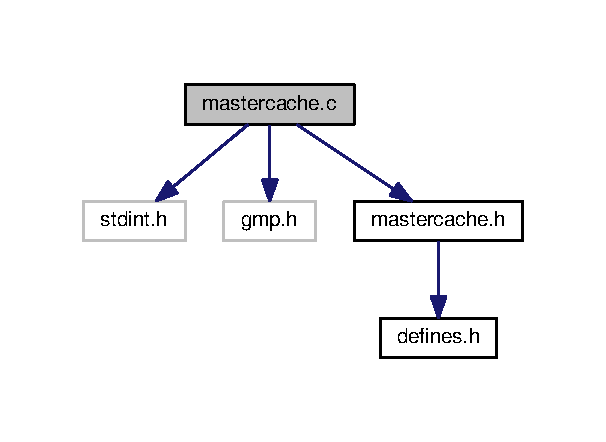
\includegraphics[width=291pt]{mastercache_8c__incl}
\end{center}
\end{figure}
\subsection*{Functions}
\begin{DoxyCompactItemize}
\item 
void \hyperlink{mastercache_8c_ad0254518fa335884d9330470e7889186}{cache\+\_\+init} (\hyperlink{structMasterCache}{Master\+Cache} $\ast$mstr, uint64\+\_\+t cache\+\_\+size)
\begin{DoxyCompactList}\small\item\em Init function for master cache. \end{DoxyCompactList}\item 
cached\+Int \hyperlink{mastercache_8c_a50d90b1940a54a27f5582e46f02483c2}{cache\+\_\+add} (\hyperlink{structMasterCache}{Master\+Cache} $\ast$mstr, mpz\+\_\+t new)
\begin{DoxyCompactList}\small\item\em add function for master cache \end{DoxyCompactList}\item 
bool \hyperlink{mastercache_8c_af3f696b0d56758825d872a5280bcfd7b}{cache\+\_\+exists} (\hyperlink{structMasterCache}{Master\+Cache} $\ast$mstr, mpz\+\_\+t element)
\begin{DoxyCompactList}\small\item\em function for master cache to check if an item exists \end{DoxyCompactList}\item 
void \hyperlink{mastercache_8c_acd42afe339ef9ef2a2c6c6733f870e07}{cache\+\_\+get} (\hyperlink{structMasterCache}{Master\+Cache} $\ast$mstr, cached\+Int element, mpz\+\_\+t result)
\begin{DoxyCompactList}\small\item\em function for master cache to get an item back from cache as mpq\+\_\+t \end{DoxyCompactList}\end{DoxyCompactItemize}


\subsection{Detailed Description}
Master Cache for caching Integers and Integer operations from gmp. 

\begin{DoxyAuthor}{Author}
Sandra Hicks 
\end{DoxyAuthor}


\subsection{Function Documentation}
\index{mastercache.\+c@{mastercache.\+c}!cache\+\_\+add@{cache\+\_\+add}}
\index{cache\+\_\+add@{cache\+\_\+add}!mastercache.\+c@{mastercache.\+c}}
\subsubsection[{\texorpdfstring{cache\+\_\+add(\+Master\+Cache $\ast$mstr, mpz\+\_\+t new)}{cache_add(MasterCache *mstr, mpz_t new)}}]{\setlength{\rightskip}{0pt plus 5cm}cached\+Int cache\+\_\+add (
\begin{DoxyParamCaption}
\item[{{\bf Master\+Cache} $\ast$}]{mstr, }
\item[{mpz\+\_\+t}]{new}
\end{DoxyParamCaption}
)}\hypertarget{mastercache_8c_a50d90b1940a54a27f5582e46f02483c2}{}\label{mastercache_8c_a50d90b1940a54a27f5582e46f02483c2}


add function for master cache 


\begin{DoxyParams}{Parameters}
{\em mstr} & \hyperlink{structMasterCache}{Master\+Cache} pointer \\
\hline
{\em new} & mpz\+\_\+t to be added to cache \\
\hline
\end{DoxyParams}
\index{mastercache.\+c@{mastercache.\+c}!cache\+\_\+exists@{cache\+\_\+exists}}
\index{cache\+\_\+exists@{cache\+\_\+exists}!mastercache.\+c@{mastercache.\+c}}
\subsubsection[{\texorpdfstring{cache\+\_\+exists(\+Master\+Cache $\ast$mstr, mpz\+\_\+t element)}{cache_exists(MasterCache *mstr, mpz_t element)}}]{\setlength{\rightskip}{0pt plus 5cm}bool cache\+\_\+exists (
\begin{DoxyParamCaption}
\item[{{\bf Master\+Cache} $\ast$}]{mstr, }
\item[{mpz\+\_\+t}]{element}
\end{DoxyParamCaption}
)}\hypertarget{mastercache_8c_af3f696b0d56758825d872a5280bcfd7b}{}\label{mastercache_8c_af3f696b0d56758825d872a5280bcfd7b}


function for master cache to check if an item exists 


\begin{DoxyParams}{Parameters}
{\em mstr} & \hyperlink{structMasterCache}{Master\+Cache} pointer \\
\hline
{\em element} & mpz\+\_\+t to be added to cache \\
\hline
\end{DoxyParams}
\index{mastercache.\+c@{mastercache.\+c}!cache\+\_\+get@{cache\+\_\+get}}
\index{cache\+\_\+get@{cache\+\_\+get}!mastercache.\+c@{mastercache.\+c}}
\subsubsection[{\texorpdfstring{cache\+\_\+get(\+Master\+Cache $\ast$mstr, cached\+Int element, mpz\+\_\+t result)}{cache_get(MasterCache *mstr, cachedInt element, mpz_t result)}}]{\setlength{\rightskip}{0pt plus 5cm}void cache\+\_\+get (
\begin{DoxyParamCaption}
\item[{{\bf Master\+Cache} $\ast$}]{mstr, }
\item[{cached\+Int}]{element, }
\item[{mpz\+\_\+t}]{result}
\end{DoxyParamCaption}
)}\hypertarget{mastercache_8c_acd42afe339ef9ef2a2c6c6733f870e07}{}\label{mastercache_8c_acd42afe339ef9ef2a2c6c6733f870e07}


function for master cache to get an item back from cache as mpq\+\_\+t 


\begin{DoxyParams}{Parameters}
{\em mstr} & \hyperlink{structMasterCache}{Master\+Cache} pointer \\
\hline
{\em element} & id of the element to get from cache \\
\hline
\end{DoxyParams}
\index{mastercache.\+c@{mastercache.\+c}!cache\+\_\+init@{cache\+\_\+init}}
\index{cache\+\_\+init@{cache\+\_\+init}!mastercache.\+c@{mastercache.\+c}}
\subsubsection[{\texorpdfstring{cache\+\_\+init(\+Master\+Cache $\ast$mstr, uint64\+\_\+t cache\+\_\+size)}{cache_init(MasterCache *mstr, uint64_t cache_size)}}]{\setlength{\rightskip}{0pt plus 5cm}void cache\+\_\+init (
\begin{DoxyParamCaption}
\item[{{\bf Master\+Cache} $\ast$}]{mstr, }
\item[{uint64\+\_\+t}]{cache\+\_\+size}
\end{DoxyParamCaption}
)}\hypertarget{mastercache_8c_ad0254518fa335884d9330470e7889186}{}\label{mastercache_8c_ad0254518fa335884d9330470e7889186}


Init function for master cache. 


\begin{DoxyParams}{Parameters}
{\em mstr} & \hyperlink{structMasterCache}{Master\+Cache} pointer to be initialized \\
\hline
{\em cache\+\_\+size} & size of the cache for mpz\+\_\+t \\
\hline
\end{DoxyParams}

\hypertarget{mpz__caching_8c}{}\section{mpz\+\_\+caching.\+c File Reference}
\label{mpz__caching_8c}\index{mpz\+\_\+caching.\+c@{mpz\+\_\+caching.\+c}}


cache  


{\ttfamily \#include \char`\"{}mpz\+\_\+caching.\+h\char`\"{}}\\*
{\ttfamily \#include \char`\"{}mastercache.\+h\char`\"{}}\\*
Include dependency graph for mpz\+\_\+caching.\+c\+:
\nopagebreak
\begin{figure}[H]
\begin{center}
\leavevmode
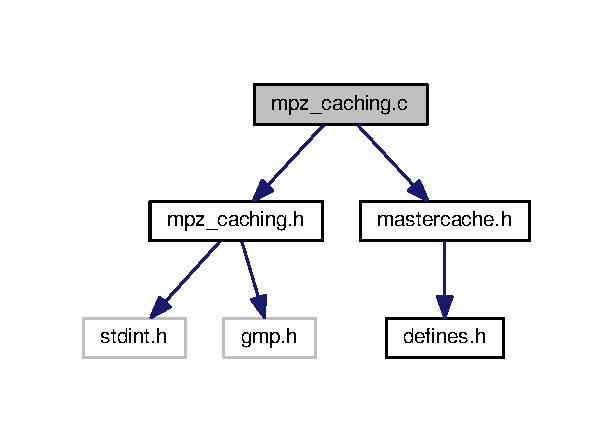
\includegraphics[width=294pt]{mpz__caching_8c__incl}
\end{center}
\end{figure}
\subsection*{Functions}
\begin{DoxyCompactItemize}
\item 
void {\bfseries init\+\_\+mpz\+\_\+cache} (int64\+\_\+t size, \hyperlink{structcached__mpz__t}{cached\+\_\+mpz\+\_\+t} $\ast$result)\hypertarget{mpz__caching_8c_a109c49f18d6466a6ede1e21ac45f090c}{}\label{mpz__caching_8c_a109c49f18d6466a6ede1e21ac45f090c}

\end{DoxyCompactItemize}


\subsection{Detailed Description}
cache 

\begin{DoxyAuthor}{Author}
Sandra Hicks 
\end{DoxyAuthor}

\hypertarget{overflow__detection_8c}{}\section{overflow\+\_\+detection.\+c File Reference}
\label{overflow__detection_8c}\index{overflow\+\_\+detection.\+c@{overflow\+\_\+detection.\+c}}


Functions to detect overflows in integer operations.  


{\ttfamily \#include $<$stdint.\+h$>$}\\*
{\ttfamily \#include \char`\"{}overflow\+\_\+detection.\+h\char`\"{}}\\*
{\ttfamily \#include \char`\"{}defines.\+h\char`\"{}}\\*
{\ttfamily \#include $<$stdio.\+h$>$}\\*
{\ttfamily \#include $<$inttypes.\+h$>$}\\*
Include dependency graph for overflow\+\_\+detection.\+c\+:\nopagebreak
\begin{figure}[H]
\begin{center}
\leavevmode
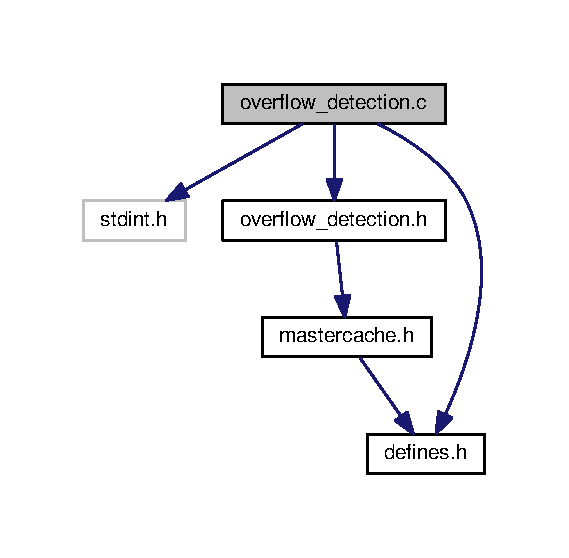
\includegraphics[width=350pt]{overflow__detection_8c__incl}
\end{center}
\end{figure}
\subsection*{Macros}
\begin{DoxyCompactItemize}
\item 
\#define \hyperlink{overflow__detection_8c_af3694ae57103552f7fba8b94e114a90f}{M\+A\+X\+B\+IT}~62
\end{DoxyCompactItemize}
\subsection*{Functions}
\begin{DoxyCompactItemize}
\item 
uint32\+\_\+t \hyperlink{overflow__detection_8c_ab9ebfca4f389fbfd7518c73802739dfa}{M\+SB} (\hyperlink{mastercache_8h_a113c03970467afb459ed5ae157d0a870}{cached\+Int} val)
\item 
\hyperlink{mastercache_8h_a113c03970467afb459ed5ae157d0a870}{cached\+Int} \hyperlink{overflow__detection_8c_a069c125ad06465b64cbfe809b29ec9ce}{delete\+Id\+Bit} (\hyperlink{mastercache_8h_a113c03970467afb459ed5ae157d0a870}{cached\+Int} val)
\item 
int \hyperlink{overflow__detection_8c_a9353ddb1f8619095dfce206ab4209d3a}{addition\+Overflow} (\hyperlink{mastercache_8h_a113c03970467afb459ed5ae157d0a870}{cached\+Int} op1, \hyperlink{mastercache_8h_a113c03970467afb459ed5ae157d0a870}{cached\+Int} op2)
\begin{DoxyCompactList}\small\item\em function to predict if an addition will overflow \end{DoxyCompactList}\item 
int \hyperlink{overflow__detection_8c_a3d152657eff6ecfd62713f7252beb0fe}{multiplication\+Overflow} (\hyperlink{mastercache_8h_a113c03970467afb459ed5ae157d0a870}{cached\+Int} op1, \hyperlink{mastercache_8h_a113c03970467afb459ed5ae157d0a870}{cached\+Int} op2)
\begin{DoxyCompactList}\small\item\em function to predict if a multiplication will overflow \end{DoxyCompactList}\item 
int \hyperlink{overflow__detection_8c_a3f5d390da9ae4425c7ba83964f3b0905}{exponentiation\+Overflow} (\hyperlink{mastercache_8h_a113c03970467afb459ed5ae157d0a870}{cached\+Int} base, \hyperlink{mastercache_8h_a113c03970467afb459ed5ae157d0a870}{cached\+Int} exp)
\begin{DoxyCompactList}\small\item\em function to predict if an exponentiation will overflow \end{DoxyCompactList}\end{DoxyCompactItemize}


\subsection{Detailed Description}
Functions to detect overflows in integer operations. 

\begin{DoxyAuthor}{Author}
Sandra Hicks 
\end{DoxyAuthor}


\subsection{Macro Definition Documentation}
\index{overflow\+\_\+detection.\+c@{overflow\+\_\+detection.\+c}!M\+A\+X\+B\+IT@{M\+A\+X\+B\+IT}}
\index{M\+A\+X\+B\+IT@{M\+A\+X\+B\+IT}!overflow\+\_\+detection.\+c@{overflow\+\_\+detection.\+c}}
\subsubsection[{\texorpdfstring{M\+A\+X\+B\+IT}{MAXBIT}}]{\setlength{\rightskip}{0pt plus 5cm}\#define M\+A\+X\+B\+IT~62}\hypertarget{overflow__detection_8c_af3694ae57103552f7fba8b94e114a90f}{}\label{overflow__detection_8c_af3694ae57103552f7fba8b94e114a90f}
maximal bit to be set before overflow 

\subsection{Function Documentation}
\index{overflow\+\_\+detection.\+c@{overflow\+\_\+detection.\+c}!addition\+Overflow@{addition\+Overflow}}
\index{addition\+Overflow@{addition\+Overflow}!overflow\+\_\+detection.\+c@{overflow\+\_\+detection.\+c}}
\subsubsection[{\texorpdfstring{addition\+Overflow(cached\+Int op1, cached\+Int op2)}{additionOverflow(cachedInt op1, cachedInt op2)}}]{\setlength{\rightskip}{0pt plus 5cm}int addition\+Overflow (
\begin{DoxyParamCaption}
\item[{{\bf cached\+Int}}]{op1, }
\item[{{\bf cached\+Int}}]{op2}
\end{DoxyParamCaption}
)}\hypertarget{overflow__detection_8c_a9353ddb1f8619095dfce206ab4209d3a}{}\label{overflow__detection_8c_a9353ddb1f8619095dfce206ab4209d3a}


function to predict if an addition will overflow 


\begin{DoxyParams}{Parameters}
{\em op1} & first operator \\
\hline
{\em op2} & second operator \\
\hline
\end{DoxyParams}
\index{overflow\+\_\+detection.\+c@{overflow\+\_\+detection.\+c}!delete\+Id\+Bit@{delete\+Id\+Bit}}
\index{delete\+Id\+Bit@{delete\+Id\+Bit}!overflow\+\_\+detection.\+c@{overflow\+\_\+detection.\+c}}
\subsubsection[{\texorpdfstring{delete\+Id\+Bit(cached\+Int val)}{deleteIdBit(cachedInt val)}}]{\setlength{\rightskip}{0pt plus 5cm}{\bf cached\+Int} delete\+Id\+Bit (
\begin{DoxyParamCaption}
\item[{{\bf cached\+Int}}]{val}
\end{DoxyParamCaption}
)}\hypertarget{overflow__detection_8c_a069c125ad06465b64cbfe809b29ec9ce}{}\label{overflow__detection_8c_a069c125ad06465b64cbfe809b29ec9ce}
(for internal use only!) 
\begin{DoxyParams}{Parameters}
{\em val} & \\
\hline
\end{DoxyParams}
\begin{DoxyReturn}{Returns}

\end{DoxyReturn}
\index{overflow\+\_\+detection.\+c@{overflow\+\_\+detection.\+c}!exponentiation\+Overflow@{exponentiation\+Overflow}}
\index{exponentiation\+Overflow@{exponentiation\+Overflow}!overflow\+\_\+detection.\+c@{overflow\+\_\+detection.\+c}}
\subsubsection[{\texorpdfstring{exponentiation\+Overflow(cached\+Int base, cached\+Int exp)}{exponentiationOverflow(cachedInt base, cachedInt exp)}}]{\setlength{\rightskip}{0pt plus 5cm}int exponentiation\+Overflow (
\begin{DoxyParamCaption}
\item[{{\bf cached\+Int}}]{base, }
\item[{{\bf cached\+Int}}]{exp}
\end{DoxyParamCaption}
)}\hypertarget{overflow__detection_8c_a3f5d390da9ae4425c7ba83964f3b0905}{}\label{overflow__detection_8c_a3f5d390da9ae4425c7ba83964f3b0905}


function to predict if an exponentiation will overflow 


\begin{DoxyParams}{Parameters}
{\em base} & first operator, base \\
\hline
{\em exp} & second operator, exponent \\
\hline
\end{DoxyParams}
\index{overflow\+\_\+detection.\+c@{overflow\+\_\+detection.\+c}!M\+SB@{M\+SB}}
\index{M\+SB@{M\+SB}!overflow\+\_\+detection.\+c@{overflow\+\_\+detection.\+c}}
\subsubsection[{\texorpdfstring{M\+S\+B(cached\+Int val)}{MSB(cachedInt val)}}]{\setlength{\rightskip}{0pt plus 5cm}uint32\+\_\+t M\+SB (
\begin{DoxyParamCaption}
\item[{{\bf cached\+Int}}]{val}
\end{DoxyParamCaption}
)}\hypertarget{overflow__detection_8c_ab9ebfca4f389fbfd7518c73802739dfa}{}\label{overflow__detection_8c_ab9ebfca4f389fbfd7518c73802739dfa}
(for internal use only!) 
\begin{DoxyParams}{Parameters}
{\em val} & \\
\hline
\end{DoxyParams}
\begin{DoxyReturn}{Returns}

\end{DoxyReturn}
\index{overflow\+\_\+detection.\+c@{overflow\+\_\+detection.\+c}!multiplication\+Overflow@{multiplication\+Overflow}}
\index{multiplication\+Overflow@{multiplication\+Overflow}!overflow\+\_\+detection.\+c@{overflow\+\_\+detection.\+c}}
\subsubsection[{\texorpdfstring{multiplication\+Overflow(cached\+Int op1, cached\+Int op2)}{multiplicationOverflow(cachedInt op1, cachedInt op2)}}]{\setlength{\rightskip}{0pt plus 5cm}int multiplication\+Overflow (
\begin{DoxyParamCaption}
\item[{{\bf cached\+Int}}]{op1, }
\item[{{\bf cached\+Int}}]{op2}
\end{DoxyParamCaption}
)}\hypertarget{overflow__detection_8c_a3d152657eff6ecfd62713f7252beb0fe}{}\label{overflow__detection_8c_a3d152657eff6ecfd62713f7252beb0fe}


function to predict if a multiplication will overflow 


\begin{DoxyParams}{Parameters}
{\em op1} & first operator \\
\hline
{\em op2} & second operator \\
\hline
\end{DoxyParams}

%--- End generated contents ---

% Index
\backmatter
\newpage
\phantomsection
\clearemptydoublepage
\addcontentsline{toc}{chapter}{Index}
\printindex

\end{document}
